% ============================================================
%  Plantilla para el Proyecto Final de Aprendizaje Automático
%  Escuela Politécnica Superior — Universidad de Alicante
%  Formato: artículo científico (una columna)
% ============================================================

\documentclass[11pt,a4paper]{article}

\usepackage[utf8]{inputenc}
\usepackage[T1]{fontenc}
\usepackage[spanish,es-tabla]{babel}
\usepackage[margin=2.5cm]{geometry}
\usepackage{amsmath}
\usepackage{amssymb}
\usepackage{bm}
\usepackage{graphicx}
\usepackage{booktabs}
\usepackage{multirow}
\usepackage{array}
\usepackage{float}
\usepackage{listings}
\usepackage{xcolor}
\usepackage[T1]{fontenc}
\usepackage{lmodern}
\usepackage{microtype}

\lstset{
    language=Python,
    basicstyle=\ttfamily\footnotesize,
    keywordstyle=\color{blue},
    commentstyle=\color{gray},
    stringstyle=\color{red!70!black},
    showstringspaces=false,
    breaklines=true,
    frame=single,
    numbers=left,
    numberstyle=\tiny\color{gray}
}

\usepackage{hyperref}
\hypersetup{
    colorlinks=true,
    linkcolor=blue!70!black,
    citecolor=blue!70!black,
    urlcolor=blue!70!black
}

% Configuración de bloques de orientación
\usepackage{mdframed}

\newmdenv[
  backgroundcolor=blue!6,
  linecolor=blue!50!black,
  linewidth=1pt,
  roundcorner=4pt,
  innerleftmargin=8pt,
  innerrightmargin=8pt,
  innertopmargin=6pt,
  innerbottommargin=6pt,
  skipabove=6pt,
  skipbelow=4pt
]{orientacion}

\newcommand{\orientaciontitle}{%
  {\small\bfseries\color{blue!60!black}Orientación}\par\smallskip
}

% Otros 
\usepackage{microtype}


% ============================================================
%  DATOS DEL TRABAJO 
% ============================================================

\title{
    \textbf{[Título del trabajo]}\\[4pt]
    \large [Subtítulo opcional]
}

\author{
    \textbf{[Nombre Apellido1]}\thanks{\texttt{[email1@alu.ua.es]}}
    \quad
    \textbf{[Nombre Apellido2]}\thanks{\texttt{[email2@alu.ua.es]}}
    \quad
    \textbf{[Nombre Apellido3]}\thanks{\texttt{[email3@alu.ua.es]}}
    \\[4pt]
    \small Grado en Ingeniería en Inteligencia Artificial
    --- Escuela Politécnica Superior, Universidad de Alicante\\
    \small Aprendizaje Avanzado --- Curso 2025/2026
}

\date{}

% ============================================================

\begin{document}

\maketitle
\thispagestyle{empty}

% Abstract 

\begin{abstract}
\textit{Resumen del trabajo en 150--250 palabras. Debe incluir:
(1)~el problema abordado y su relevancia real,
(2)~el \textit{dataset} utilizado,
(3)~las problemáticas identificadas y las técnicas aplicadas,
(4)~los resultados principales.
\textbf{Escríbelo al final, una vez completado el trabajo.}}
\end{abstract}

\smallskip
\noindent\textbf{Palabras clave:} aprendizaje automático, [problemática 1], [problemática 2], [dataset], [otra palabra clave].

\tableofcontents
\newpage


% ============================================================
\section{Introducción}
% ============================================================

\begin{orientacion}
\orientaciontitle
\textit{La introducción debe responder a cuatro preguntas: (1)~?`Cuál es el problema y por qué es relevante? (2)~?`Qué implicaciones éticas, sociales o legales tiene? (3)~?`Qué se propone hacer este trabajo? (4)~?`Cómo se organiza el resto del documento? No es un resumen del trabajo, sino una motivación y contextualización.}
\end{orientacion}

En los últimos años, el uso de modelos de aprendizaje automático en contextos de alto impacto social ha crecido de forma significativa, especialmente en áreas relacionadas con la toma de decisiones públicas. Uno de los ámbitos más sensibles es el sistema judicial, donde algoritmos de predicción se utilizan o se proponen como herramientas de apoyo para estimar la probabilidad de reincidencia de individuos dentro del sistema penal. Estos sistemas pueden influir en decisiones críticas como la concesión de libertad condicional, la asignación de recursos penitenciarios o la participación en programas de rehabilitación.

Sin embargo, la aplicación de estos modelos en entornos judiciales plantea desafíos fundamentales tanto técnicos como éticos. En particular, los errores de predicción pueden tener consecuencias graves a nivel individual y social: un \textit{falso positivo} puede contribuir a decisiones injustamente restrictivas, mientras que un \textit{falso negativo} puede subestimar el riesgo real de reincidencia. Además, diversos estudios han evidenciado la presencia de sesgos en los datos utilizados para entrenar estos modelos, lo que puede derivar en resultados discriminatorios hacia ciertos grupos demográficos.

En este contexto, el dataset \textit{COMPAS Recidivism} de ProPublica se ha convertido en un referente para el estudio de estas problemáticas, al poner en evidencia posibles desigualdades raciales en sistemas de predicción de riesgo. A partir de este caso, surge la necesidad de analizar no solo el rendimiento predictivo de los modelos, sino también su equidad (\textit{fairness}) y su capacidad de explicación (\textit{explainability}), aspectos clave para su posible aplicación en entornos reales.

El presente proyecto tiene como objetivo desarrollar un modelo de aprendizaje automático para la predicción de reincidencia, acompañado de un análisis crítico de sus implicaciones éticas. En particular, se abordarán dos problemáticas principales: la detección y evaluación de sesgos en las predicciones mediante métricas de equidad, y la interpretabilidad del modelo mediante técnicas de explicabilidad (\textit{XAI}), como \textit{SHAP} (\textit{SHapley Additive exPlanations}). De este modo, se busca no solo optimizar el rendimiento del modelo, sino también evaluar su transparencia, justicia y viabilidad en contextos judiciales reales.

El resto del artículo se organiza como sigue.
La Sección~\ref{sec:related} revisa el trabajo relacionado.
La Sección~\ref{sec:datos} describe el \textit{dataset} y el análisis exploratorio.
La Sección~\ref{sec:metodologia} detalla la metodología.
La Sección~\ref{sec:resultados} presenta los resultados experimentales.
La Sección~\ref{sec:discusion} discute las implicaciones.
La Sección~\ref{sec:conclusiones} concluye el trabajo.

% ============================================================
\section{Trabajo Relacionado}
\label{sec:related}
% ============================================================

\subsection{Modelos de predicción de reincidencia y el impacto de COMPAS}

La aplicación de algoritmos de aprendizaje automático (\textit{Machine Learning}, ML) en el sistema de justicia penal se ha expandido como una herramienta para reducir los altos índices de reincidencia, que en diversas jurisdicciones internacionales alcanzan el 50\%. La literatura científica ha evolucionado desde el uso de escalas estadísticas simples hacia modelos complejos que buscan optimizar la toma de decisiones sobre libertad condicional y rehabilitación. En términos de rendimiento, revisiones sistemáticas recientes sitúan el estado del arte en una precisión ($ACC$) media de 0.81 y un área bajo la curva ($AUC$) de 0.74 \cite{travaini2022machine}. 

Diversos estudios han explorado una amplia gama de arquitecturas para maximizar esta capacidad predictiva. Por ejemplo, Duwe y Kim (2017) emplearon algoritmos de \textit{LogitBoost} sobre el \textit{dataset} MnSTARR+, obteniendo un $ACC$ de 0.82 y un $AUC$ de 0.78 \cite{duwe2017out}. Por su parte, Singh y Mohapatra (2021) propusieron un modelo de ensamble (\textit{Ensemble Learning}) combinando clasificadores Bayesiano, KNN y SVM, alcanzando un $ACC$ de 0.87 en poblaciones de delincuentes primerizos \cite{singh2021development}. En contextos institucionales específicos, Butsara et al. (2019) reportaron precisiones de hasta 0.90 mediante regresión logística aplicada a internos en Tailandia \cite{butsara2019predicting}. Asimismo, para tipos de delitos específicos como el sexual, trabajos basados en Análisis Discriminante Lineal (LDA) y \textit{Random Forest} han reportado valores de $ACC$ de hasta 0.96 y $AUC$ de 0.78, respectivamente \cite{tollenaar2013method, salo2019predictive}. A pesar de estos avances técnicos, el caso de COMPAS ha puesto de manifiesto que un alto rendimiento no excluye la presencia de sesgos críticos, impulsando la necesidad de evaluar la equidad junto con la precisión \cite{angwin2016machine, karimi2021enhancing}.

En este marco, el uso del \textit{dataset} COMPAS personifica la tensión entre la eficacia técnica y la integridad ética, tras la investigación de ProPublica \cite{angwin2016machine} que evidenció disparidades críticas a pesar de los rendimientos alcanzados. Si bien se han reportado precisiones elevadas con arquitecturas avanzadas, estudios comparativos indican que modelos interpretables como la regresión logística ---frecuentemente utilizada en este dominio--- presentan una validez predictiva y un rendimiento similares a algoritmos de ``caja negra'' como \textit{Random Forest}. Esta falta de superioridad empírica de los modelos complejos, sumada a su diseño inaccesible para el usuario humano, subraya la necesidad de transitar hacia algoritmos transparentes o técnicas de \textit{Explainable AI} (XAI) que permitan discernir cómo influyen individualmente variables como la etnia o la edad en la evaluación final del riesgo.

\subsection{Equidad algorítmica y mitigación de sesgos}

El principal desafío identificado en la literatura no reside únicamente en la capacidad predictiva, sino en la presencia de sesgos discriminatorios, particularmente raciales y de edad. Diversas investigaciones han señalado que estos sesgos pueden heredarse de métodos de recolección de datos sesgados o de un preprocesamiento inadecuado, factores que influyen significativamente en el rendimiento final del modelo. 

El enfoque actual en el estado del arte, ejemplificado por trabajos como los de Karimi-Haghighi y Castillo \cite{karimi2021enhancing}, se centra en integrar métricas de equidad (\textit{fairness}) directamente en el ciclo de vida del modelo. No obstante, una limitación crítica en muchos estudios previos es la falta de explicitud sobre el proceso de preprocesamiento, lo que dificulta la comparabilidad entre diferentes técnicas de mitigación de sesgo.

\subsection{Explicabilidad (XAI) en el entorno judicial}

La naturaleza de ``caja negra'' de muchos modelos avanzados de aprendizaje automático constituye una barrera crítica en el sistema judicial, ya que impide evaluar si la predicción de riesgo cumple con principios de justicia y debido proceso. Según la taxonomía establecida por Arrieta et al. \cite{arrieta2020explainable}, la explicabilidad no debe entenderse como un concepto unívoco, sino como una propiedad dependiente de la \textit{audiencia} (jueces, abogados o acusados), quienes requieren distintos niveles de transparencia técnica y comprensibilidad para validar las decisiones del sistema.

En este ámbito, el estado del arte distingue entre modelos \textbf{intrínsecamente transparentes} --- que cumplen con propiedades de simulatabilidad, decomposabilidad y transparencia algorítmica--- y técnicas de \textbf{explicabilidad post-hoc} \cite{arrieta2020explainable}. Estas últimas son esenciales cuando se emplean algoritmos de alta complejidad (como \textit{XGBoost} o Redes Neuronales) para predecir la reincidencia, permitiendo iluminar el proceso de decisión sin sacrificar el rendimiento predictivo.

Dentro de los métodos \textit{post-hoc}, la técnica \textit{SHAP} (\textit{SHapley Additive exPlanations}) se ha consolidado como el estándar para cuantificar la contribución de cada variable. No obstante, una limitación significativa de su implementación original (\textit{Kernel SHAP}) es el supuesto de independencia entre las características. Como demuestran Aas et al. \cite{aas2021explaining}, en entornos judiciales donde las variables socioeconómicas y delictivas suelen presentar una alta correlación, ignorar estas dependencias puede derivar en explicaciones inexactas o sesgadas.

Para abordar este desafío, la literatura reciente propone extensiones de \textit{SHAP} que incorporan la dependencia de variables mediante el uso de \textbf{Cópulas Gaussianas} y \textbf{distribuciones condicionales empíricas} \cite{aas2021explaining}. Estas técnicas permiten una descomposición del riesgo más fiel a la realidad delictiva, facilitando incluso la \textbf{agrupación (clustering)} de contribuciones de variables dependientes para ofrecer una visión más clara y accionable a los operadores jurídicos.

% ============================================================
\section{Descripción del Problema y los Datos}
\label{sec:datos}
% ============================================================

\subsection{Definición formal de la tarea}

\begin{orientacion}
\orientaciontitle
\textit{Define formalmente la tarea de aprendizaje: tipo de tarea (clasificación, regresión\ldots), espacio de entrada y salida, y función objetivo. Por ejemplo: dado un vector de \textit{features} $\bm{x} \in \mathbb{R}^d$, aprender $f\colon \mathbb{R}^d \to \mathcal{Y}$ que minimiza $\mathcal{L}(f) = \mathbb{E}_{(\bm{x},y)\sim P}[\ell(f(\bm{x}),y)]$.}
\end{orientacion}

El problema abordado en este trabajo se enmarca dentro del aprendizaje supervisado, concretamente como una tarea de \textbf{clasificación binaria}. 


Sea un espacio de entrada $\mathcal{X} \subseteq \mathbb{R}^d$, donde cada vector de características $\bm{x} \in \mathcal{X}$ representa el perfil de un individuo procesado por el sistema judicial. Definimos el espacio de salida o variable objetivo como $\mathcal{Y} = \{0, 1\}$, donde $y = 1$ indica que el individuo reincide en un plazo de dos años (\textit{two-year recidivism}) y $y = 0$ indica que no lo hace. Adicionalmente, denotamos por $A \in \mathcal{A}$ al atributo sensible o protegido presente en el espacio de entrada (en nuestro caso, la raza del individuo), donde $\mathcal{A}$ representa los posibles grupos demográficos (por ejemplo, afroamericano o caucásico).

El objetivo principal del sistema es aprender una función predictiva $f\colon \mathcal{X} \to [0,1]$ que estime la probabilidad de reincidencia $\hat{y} = P(y=1 \mid \bm{x})$, minimizando el riesgo esperado respecto a una función de pérdida $\ell$:

$$ \mathcal{L}(f) = \mathbb{E}_{(\bm{x},y)\sim P}[\ell(f(\bm{x}), y)] $$

Sin embargo, dado el alto impacto social de las decisiones judiciales, la optimización tradicional del modelo predictivo está sujeta a restricciones de \textbf{equidad algorítmica} (\textit{fairness}). Por lo tanto, el objetivo de la tarea se reformula como un problema de optimización restringida, donde se busca minimizar la pérdida $\mathcal{L}(f)$ garantizando simultáneamente que el modelo cumpla con una métrica de equidad predefinida. Por ejemplo, si se busca optimizar bajo el criterio de Paridad Demográfica (\textit{Demographic Parity}), la predicción del modelo debe ser estadísticamente independiente del atributo sensible:

$$ P(\hat{y} = 1 \mid A = a) = P(\hat{y} = 1 \mid A = b) \quad \forall a, b \in \mathcal{A} $$

De este modo, la tarea no se limita a maximizar el rendimiento predictivo (precisión), sino a explorar empíricamente el compromiso (\textit{trade-off}) entre la precisión y la equidad algorítmica, incorporando posteriormente técnicas de explicabilidad (XAI) para auditar las predicciones $\hat{y}$ a nivel global y local.

\subsection{Dataset}

\begin{orientacion}
\orientaciontitle
\textit{Describe el \textit{dataset}: origen, licencia, número de instancias, número de \textit{features}, variable objetivo y distribución de clases. Incluye también las consideraciones éticas sobre su uso: ?`quiénes son los individuos representados?, ?`cómo se recogieron los datos?, ?`hay sesgos de selección conocidos?}
\end{orientacion}

La Tabla~\ref{tab:dataset} resume las características principales del \textit{dataset} utilizado.

\begin{table}[H]
\centering
\caption{Características del \textit{dataset} COMPAS original.}
\label{tab:dataset}
\small
\begin{tabular}{@{}lp{10cm}@{}}
\toprule
\textbf{Característica} & \textbf{Valor} \\
\midrule
Fuente / enlace           & ProPublica (repositorio oficial en GitHub) \\
Número de instancias      & 7214 registros originales[cite: 1] (se reducen a 6167 tras la limpieza). \\
Número de \textit{features} & 53 variables originales[cite: 1] (se seleccionan 13 relevantes para el modelado). \\
Variable objetivo         & \texttt{two\_year\_recid}[cite: 1] (Binaria: 1 = reincide, 0 = no reincide). \\
Distribución de clases & Aprox. 55\,\% clase 0 / 45\,\% clase 1 (en el subconjunto final filtrado). \\
Valores ausentes          & Sí, el 18.6\,\% de las celdas totales están vacías[cite: 1]. Estrategia: Eliminación de columnas con alto porcentaje de nulos (ej. \texttt{c\_arrest\_date} con 84.2\,\%[cite: 1]) y filtrado de filas mediante eliminación por lista (\textit{listwise deletion}). \\
Licencia                  & Open Data / Dominio público. \\
\bottomrule
\end{tabular}
\end{table}

\subsection{Análisis exploratorio (EDA)}

El preprocesamiento inicial del conjunto de datos original reveló un alto volumen de valores ausentes (NaNs) y variables problemáticas. Se procedió a descartar todas las columnas con un porcentaje de nulos superior al 80\,\%, así como aquellas variables con el prefijo \texttt{r\_}, asociadas a la reincidencia posterior, para evitar la introducción de sesgos por \textit{data leakage}. Además, se aplicaron los filtros metodológicos del estudio de ProPublica (desfase temporal razonable entre arresto y evaluación, existencia de seguimiento real, exclusión de infracciones de tráfico ordinarias y exigencia de un veredicto válido emitido por el sistema COMPAS). La decisión de eliminar los valores nulos residuales en lugar de reconstruirlos mediante técnicas de imputación se fundamenta en un principio ético: en el contexto de los Sistemas de Soporte a la Decisión Judicial, la reconstrucción sintética de historiales penales resulta inaceptable, debiendo el modelo basarse de forma exclusiva en hechos fácticos y fehacientes.

Una vez saneado el \textit{dataset}, el análisis univariado (Figura \ref{fig:eda_univariado}) mostró una distribución relativamente equilibrada de la variable objetivo (\texttt{two\_year\_recid}), lo que indica que no será estrictamente necesario aplicar técnicas de balanceo sintético de clases. Asimismo, la distribución de la variable demográfica sensible (\texttt{race}) refleja que la muestra está compuesta mayoritariamente por individuos afroamericanos y caucásicos.

\begin{figure}[H]
    \centering
    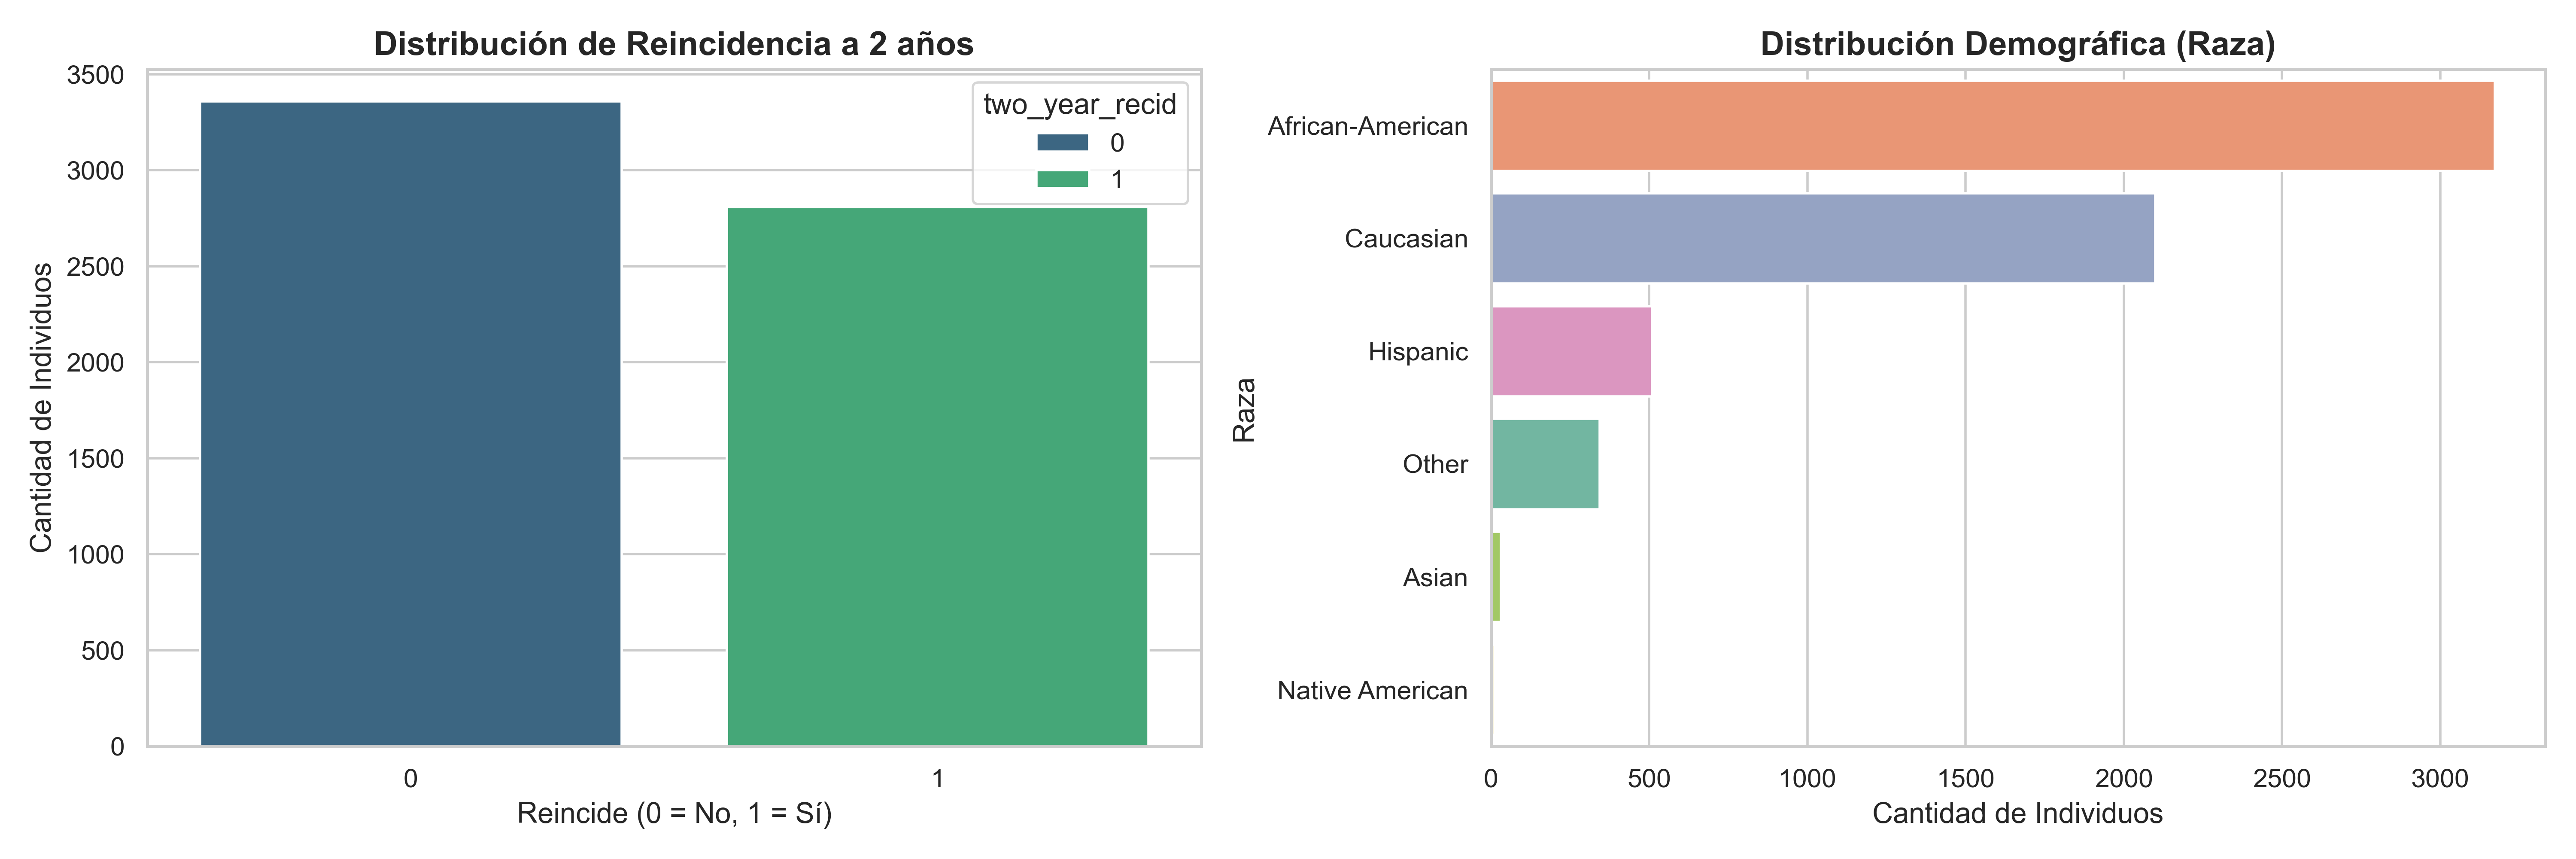
\includegraphics[width=\textwidth]{Images/eda_univariado.png}
    \caption{Análisis univariado: Distribución de la variable objetivo (reincidencia a dos años) y de la variable protegida (raza).}
    \label{fig:eda_univariado}
\end{figure}

No obstante, la problemática central del estudio afloró al cruzar la evaluación de riesgo original del sistema COMPAS (\texttt{decile\_score}) con dicha variable protegida. Como se observa en la Figura \ref{fig:eda_sesgo_racial}, la población caucásica concentra sus evaluaciones mayoritariamente en los niveles de riesgo más bajos, cayendo drásticamente en los deciles superiores. Por el contrario, la población afroamericana presenta una distribución mucho más uniforme, manteniendo frecuencias de clasificación alarmantemente altas en los niveles de riesgo máximo (deciles 8, 9 y 10).

\begin{figure}[H]
    \centering
    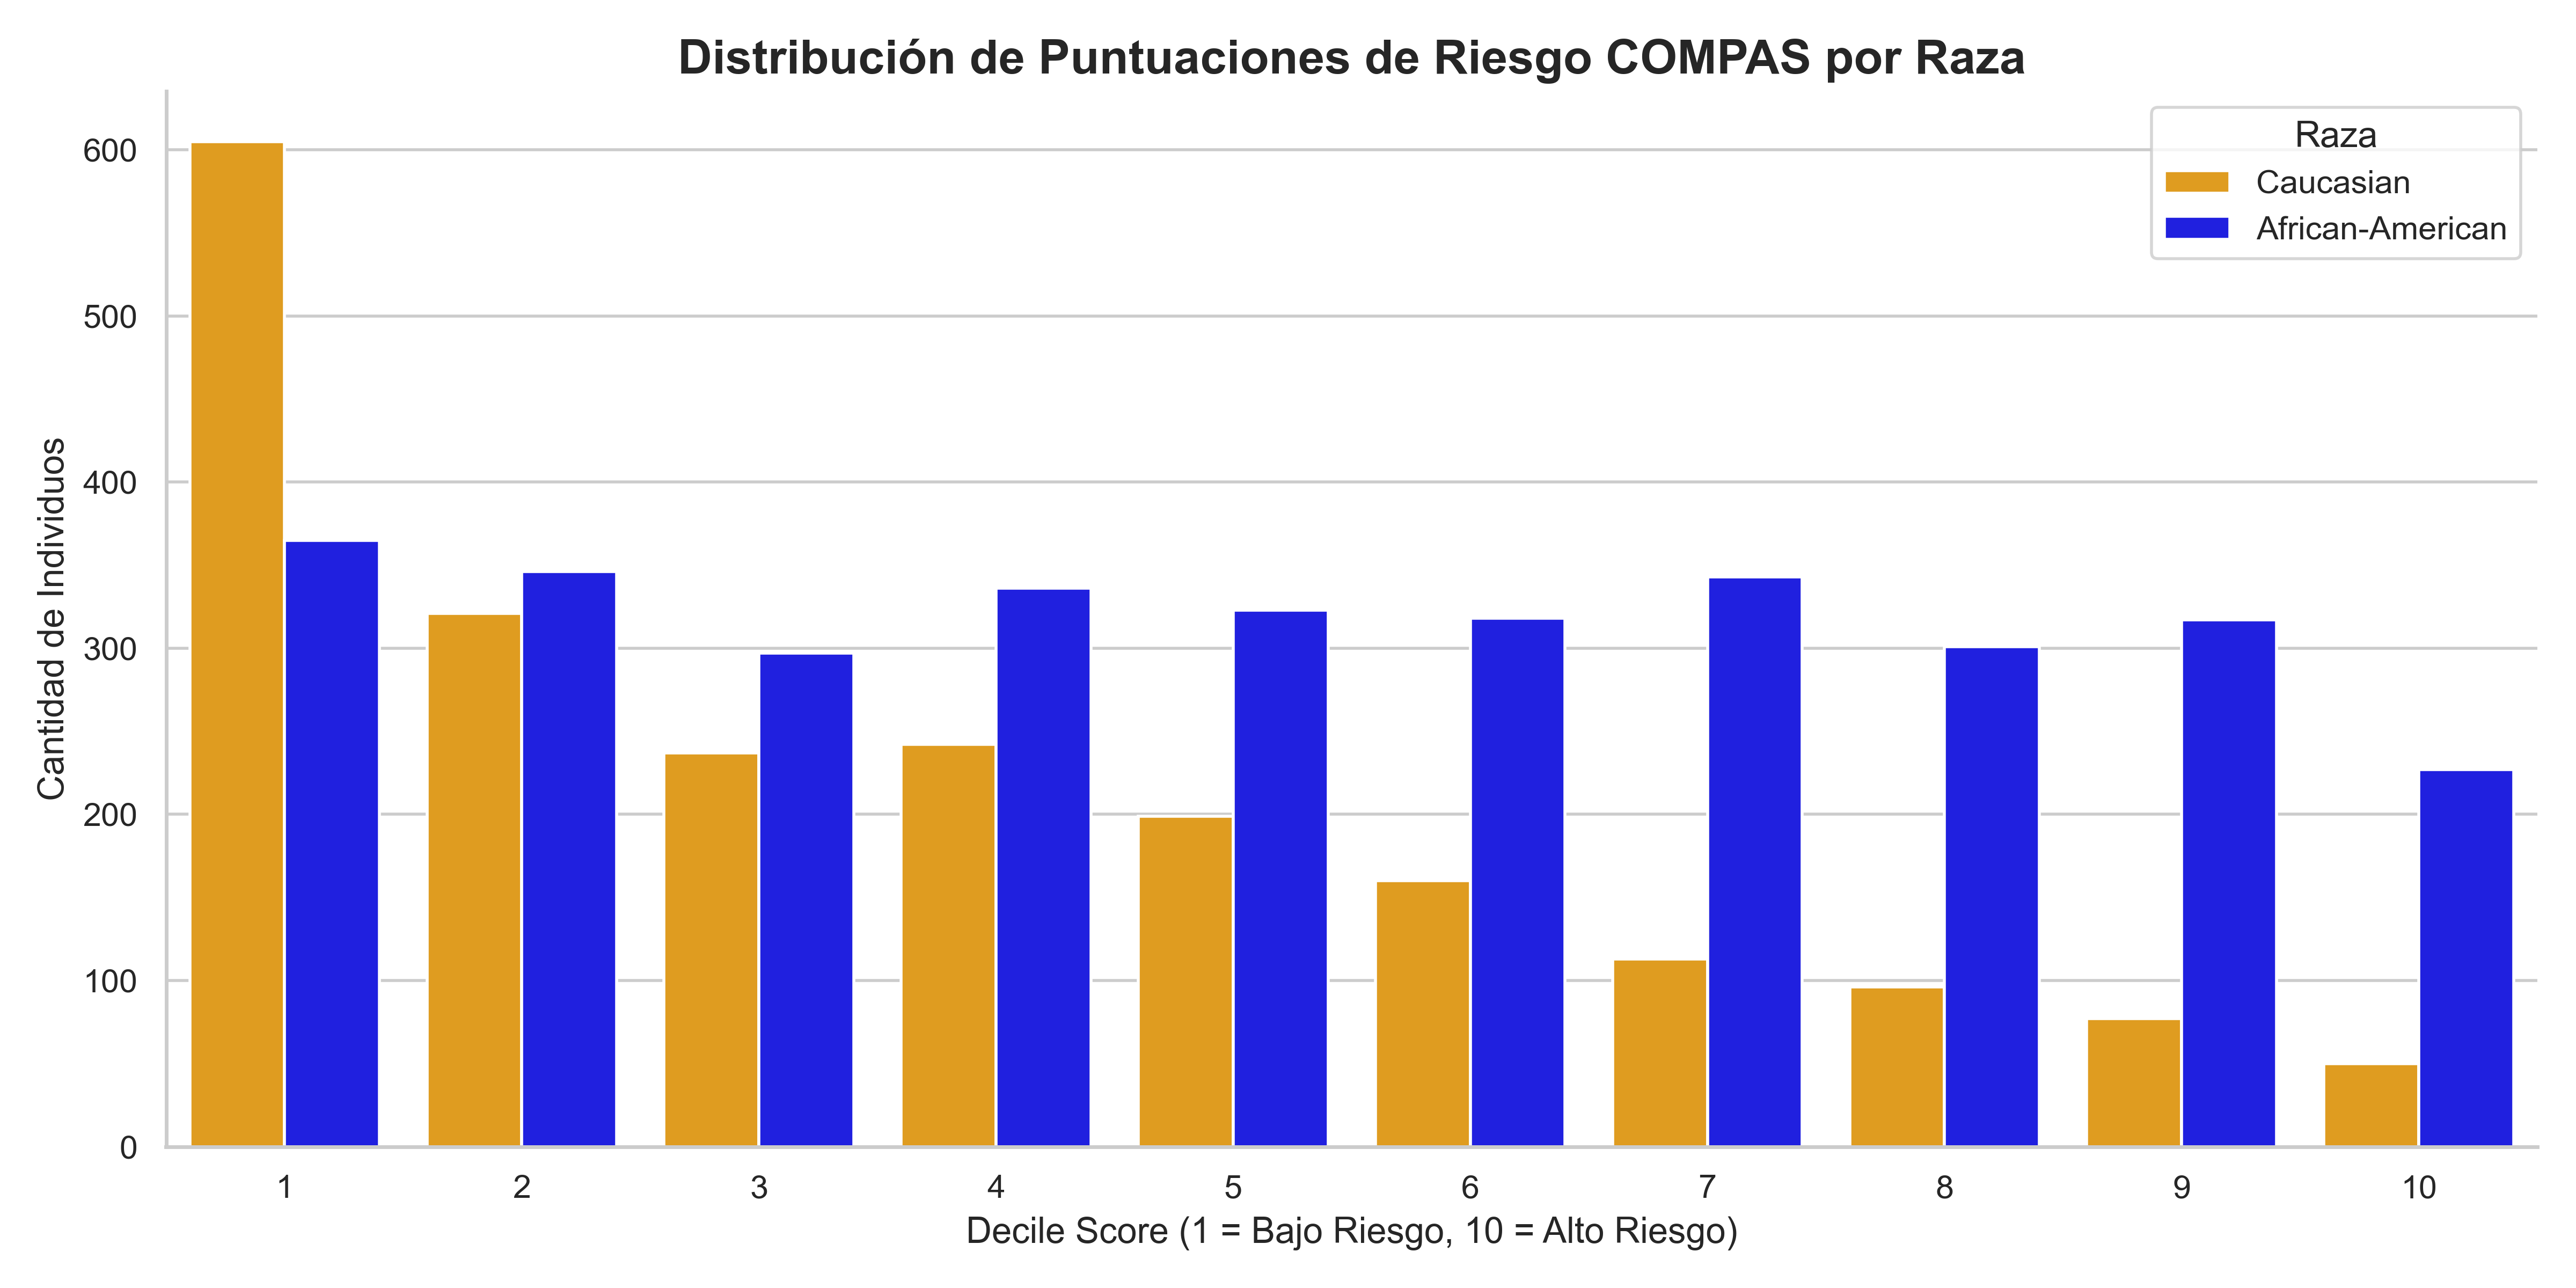
\includegraphics[width=0.85\textwidth]{Images/eda_sesgo_racial.png}
    \caption{Distribución del nivel de riesgo (\textit{Decile Score}) asignado por COMPAS segmentado por los dos grupos demográficos mayoritarios.}
    \label{fig:eda_sesgo_racial}
\end{figure}

La matriz de correlación (Figura \ref{fig:eda_correlacion}) confirma las hipótesis planteadas sobre la naturaleza del \textit{dataset} y sus sesgos intrínsecos. Por un lado, se valida la coherencia predictiva general: el historial delictivo adulto (\texttt{priors\_count}) y la edad (\texttt{age}) son los factores que mayor peso tienen en la puntuación de riesgo del sistema original (\texttt{decile\_score}), con correlaciones de $0.45$ y $-0.40$ respectivamente. Sin embargo, el hallazgo más crítico reside en la interacción entre la variable protegida y las predicciones del algoritmo. La matriz revela una disparidad evidente: la pertenencia al grupo demográfico afroamericano presenta una correlación positiva ($0.31$) con la puntuación de riesgo, mientras que para la población caucásica la correlación es negativa ($-0.20$). Estas métricas justifican plenamente la necesidad de aplicar técnicas de mitigación algorítmica (\textit{Fairness}) en el desarrollo del nuevo sistema.

\begin{figure}[H]
    \centering
    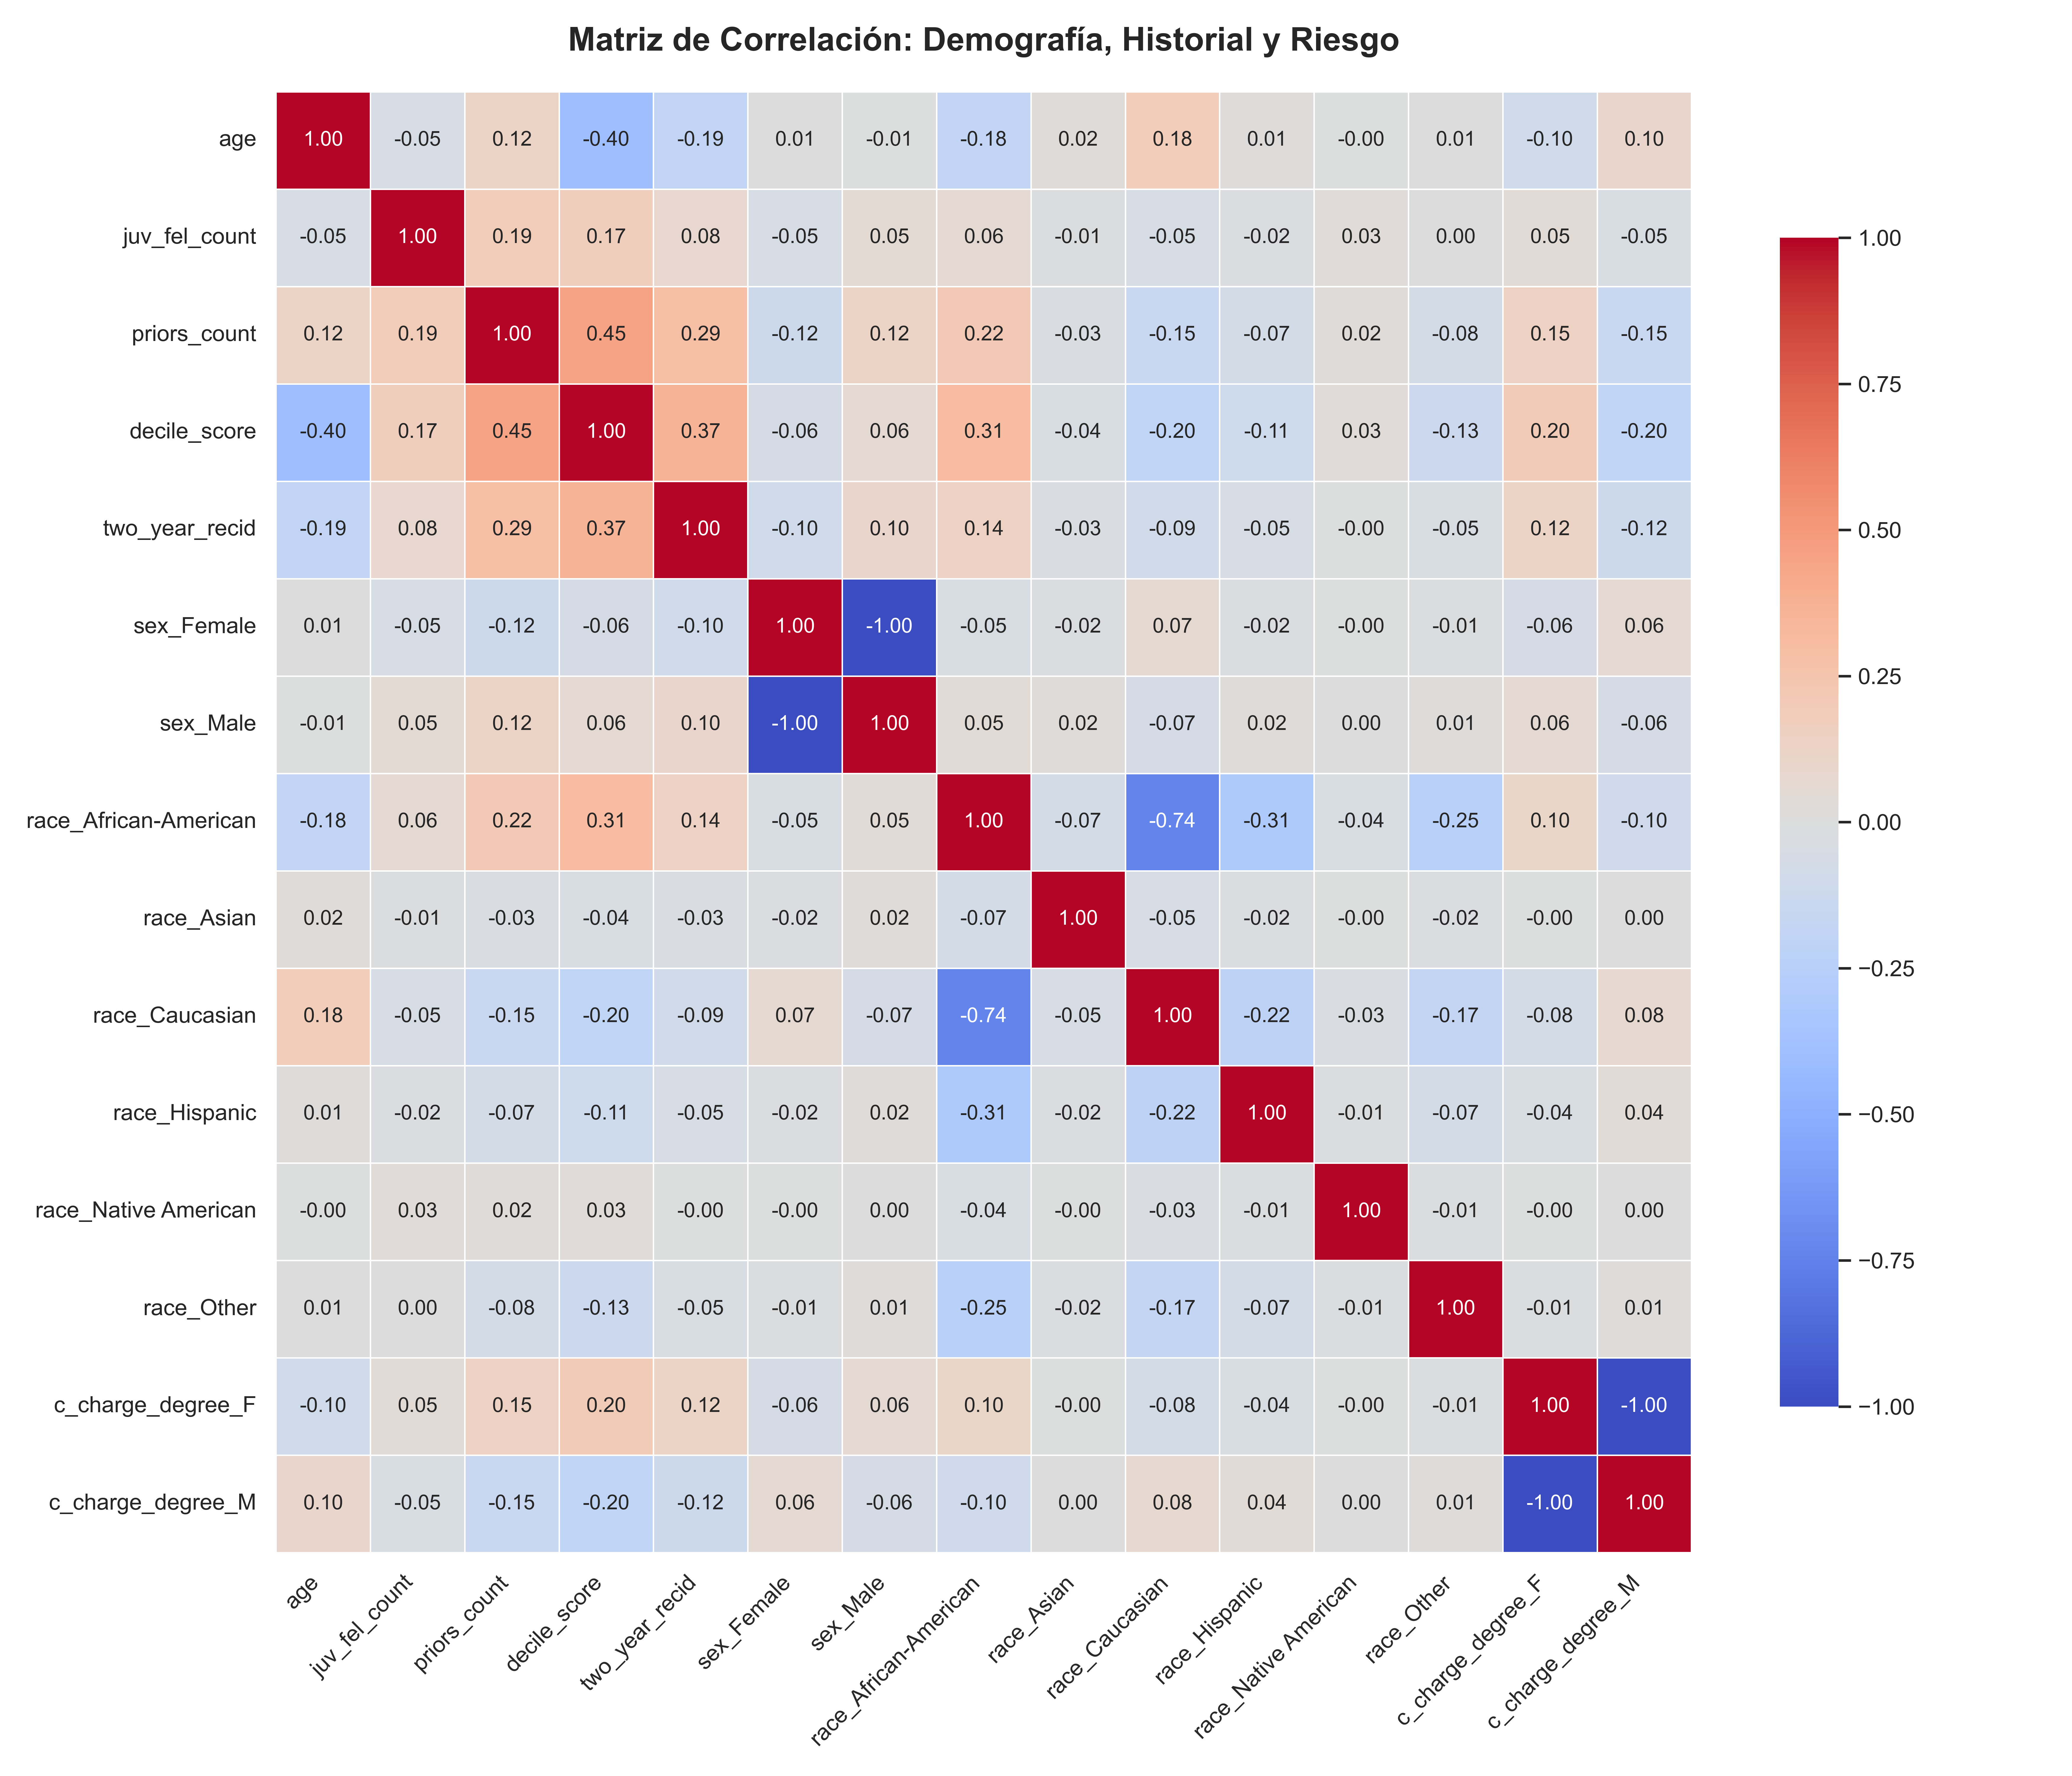
\includegraphics[width=0.9\textwidth]{Images/eda_correlacion.png}
    \caption{Matriz de correlación destacando las interacciones entre historial delictivo, atributos protegidos y la evaluación del sistema.}
    \label{fig:eda_correlacion}
\end{figure}

Para profundizar en las dos variables de mayor impacto predictivo, se analizó su densidad en función de la variable objetivo (Figura \ref{fig:eda_densidades}). Las curvas demuestran visualmente cómo la madurez del individuo mitiga sustancialmente la probabilidad de volver a delinquir (concentrando a los reincidentes en las franjas más jóvenes), mientras que la acumulación de arrestos previos ensancha significativamente la curva de densidad hacia la reincidencia efectiva.

\begin{figure}[H]
    \centering
    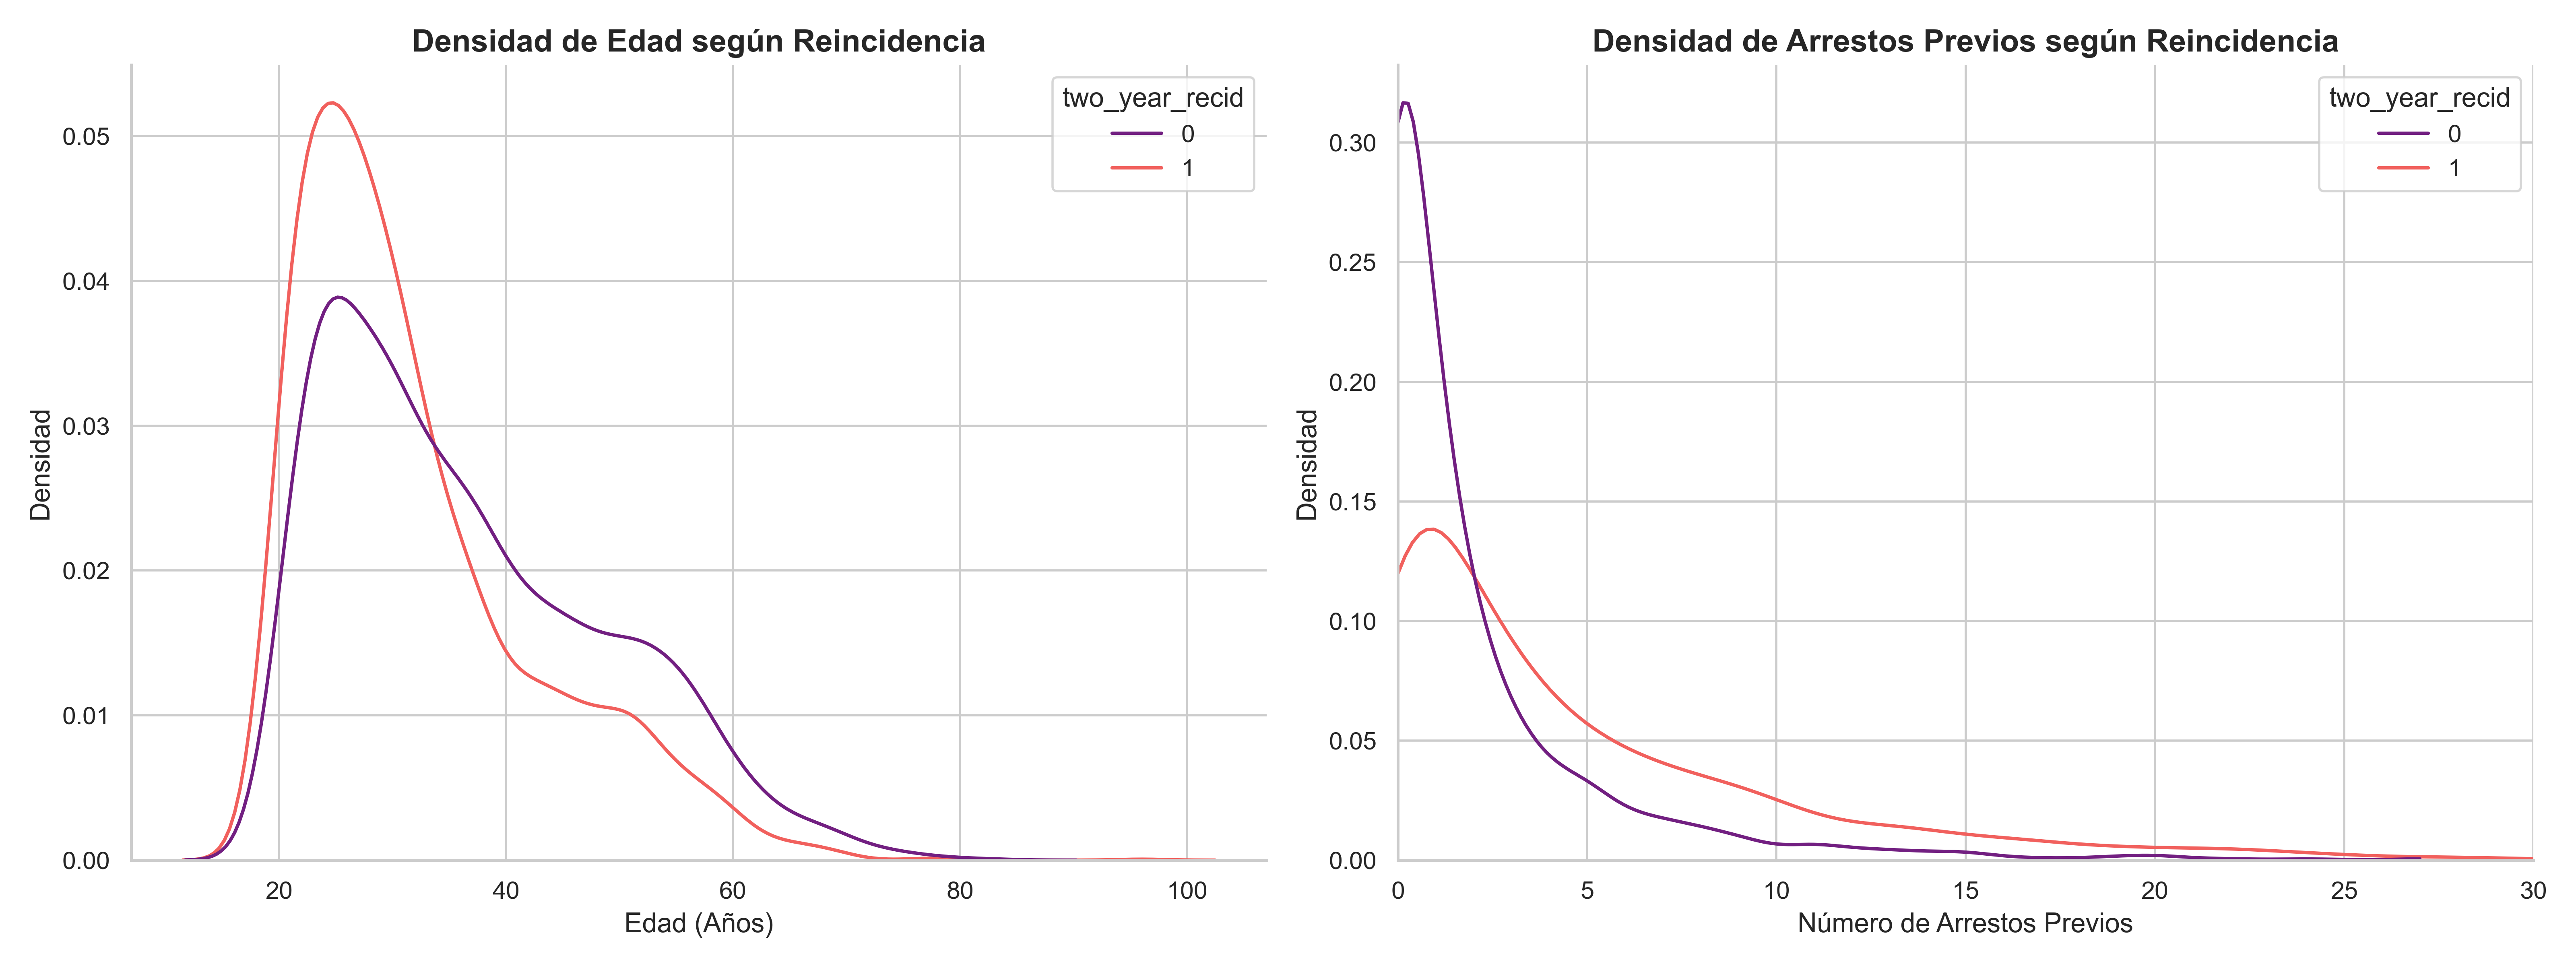
\includegraphics[width=\textwidth]{Images/eda_densidades_edad_priors.png}
    \caption{Análisis de densidad bivariado de las variables \texttt{age} y \texttt{priors\_count} segmentadas por reincidencia.}
    \label{fig:eda_densidades}
\end{figure}

Finalmente, se abordó el estudio de la dispersión de los datos (Figura \ref{fig:eda_outliers}). En las imágenes analizadas se observa un comportamiento demográfico natural en la variable de la edad, ya que presenta valores atípicos (\textit{outliers}) lógicos a partir de los 70 años. En el caso de los conteos juveniles y de arrestos previos, las distribuciones muestran cómo la mayoría de los acusados se concentra en cero o en muy pocos delitos previos. Sin embargo, existe una cola larga evidente: un grupo reducido pero significativo de reincidentes crónicos que superan el límite superior del rango intercuartílico (IQR), llegando a acumular hasta 40 arrestos previos en su etapa adulta o 20 delitos graves en su etapa juvenil.

\begin{figure}[H]
    \centering
    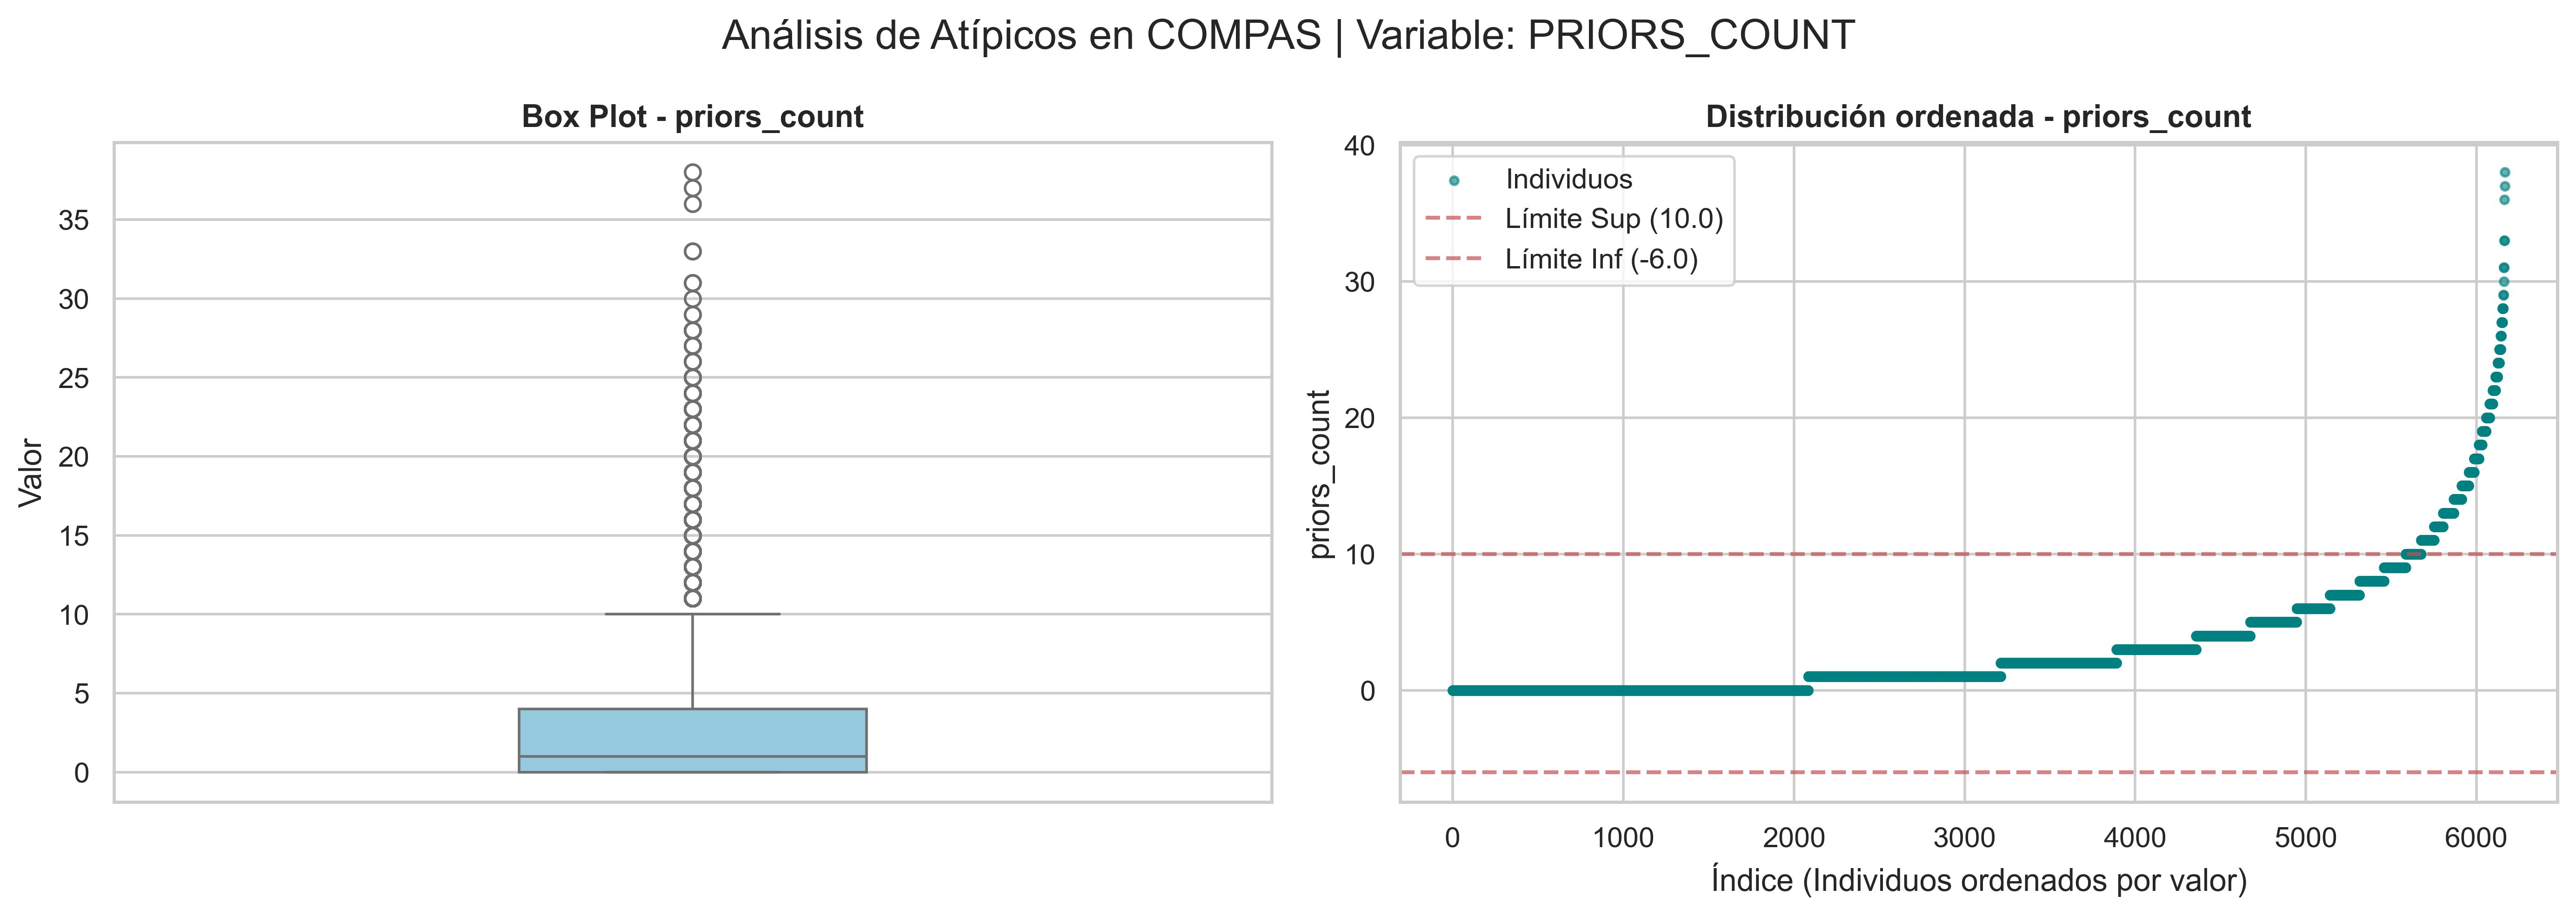
\includegraphics[width=0.95\textwidth]{Images/eda_outliers_priors_count.png}
    \caption{Análisis de valores atípicos para la variable \texttt{priors\_count}. A la izquierda, el \textit{Box Plot} identifica la mediana y el rango intercuartílico; a la derecha, el \textit{Scatter Plot} ordenado muestra cómo los reincidentes crónicos superan significativamente el límite superior estadístico.}
    \label{fig:eda_outliers}
\end{figure}

Dado que no existen \textit{outliers} que deriven de errores de recolección en el \textit{dataset}, no se eliminó a ningún individuo, ya que representan perfiles criminalísticos reales. Además, al basarse el nuevo modelo predictivo en algoritmos de tipo Árbol (como \textit{Random Forest}), se descartó la aplicación de técnicas de capeo (\textit{clipping}); la naturaleza de estos algoritmos permite definir fronteras de partición eficaces sin verse distorsionados por la magnitud extrema del historial delictivo.

A modo de conclusión de esta fase exploratoria, todas las decisiones metodológicas justificadas (filtros de calidad oficial, tratamiento estricto de nulos, exclusión de variables con riesgo de \textit{data leakage} y selección de atributos) se han encapsulado en una única función modular de preprocesamiento (\texttt{load\_and\_clean\_compas}). Esta unificación garantiza la reproducibilidad del experimento, previniendo errores manuales y asegurando que las fases posteriores de \textit{Machine Learning} operen bajo los más estrictos estándares de rigor estadístico e integridad ética.

\subsection{Problemáticas identificadas}

\begin{orientacion}
\orientaciontitle
\textit{Justifica aquí qué problemáticas son relevantes para este problema concreto. La argumentación debe basarse en: (1)~el contexto de uso real del sistema (?`quién usa el modelo?, ?`sobre quién toma decisiones?), (2)~las características del \textit{dataset} (?`hay atributos sensibles?, ?`está desbalanceado?), y (3)~las obligaciones legales aplicables (RGPD, AI Act).}
\end{orientacion}

A partir del análisis del \textit{dataset} y del contexto de uso del sistema en el ámbito penal, se han identificado las siguientes problemáticas críticas que deben ser abordadas para garantizar un despliegue ético y técnico:

\begin{itemize}
    \item \textbf{Sesgo Algorítmico y Falta de Equidad (\textit{Fairness}):} 
    El contexto de uso real del sistema implica la toma de decisiones que afectan directamente a la libertad fundamental de los individuos. El \textit{dataset} COMPAS contiene atributos sensibles explícitos, principalmente la raza (\textit{race}), que han demostrado históricamente ser fuentes de disparidad en las tasas de error de falsos positivos entre diferentes grupos demográficos. 
    Desde una perspectiva legal, el Reglamento de Inteligencia Artificial de la UE (\textit{AI Act}) clasifica los sistemas de evaluación de riesgos en la justicia como de \textbf{alto riesgo} (Anexo III). Esto impone la obligación estricta de implementar medidas de control de sesgos para evitar discriminaciones prohibidas por la Carta de los Derechos Fundamentales de la UE y el RGPD, los cuales exigen que el tratamiento de datos no resulte en resultados discriminatorios por motivos de origen étnico o racial.

    \item \textbf{Opacidad del Modelo y Necesidad de Explicabilidad (\textit{Explainability}):} 
    Dada la complejidad de las interacciones entre las variables socioeconómicas y los antecedentes penales en el \textit{dataset} (ej. la correlación entre \textit{priors\_count} y \textit{age}), los modelos con mayor rendimiento predictivo suelen operar como ``cajas negras''. En un entorno judicial, el derecho al debido proceso exige que cualquier decisión automatizada sea justificable y comprensible para las partes implicadas (jueces, abogados y acusados). 
    La problemática reside en la tensión entre la precisión técnica y la transparencia operativa. Bajo el RGPD (Art. 22), los ciudadanos tienen el derecho a recibir una \textbf{explicación significativa} sobre la lógica aplicada en decisiones automatizadas que produzcan efectos jurídicos. Por tanto, es imperativo aplicar técnicas de XAI que permitan descomponer la influencia de cada variable en la predicción individual de riesgo para garantizar la seguridad jurídica del sistema.
\end{itemize}


% ============================================================
\section{Metodología}
\label{sec:metodologia}
% ============================================================

\begin{orientacion}
\orientaciontitle
\textit{Esta sección debe ser suficientemente detallada para que el trabajo sea reproducible. Describe el \textit{pipeline} completo, justifica cada decisión de dise\~{n}o, e incluye la formulación matemática de las técnicas que lo requieran.}
\end{orientacion}

\subsection{Preprocesamiento de Datos}
\label{subsec:preprocesamiento}

Tras la fase de Análisis Exploratorio de Datos (EDA) y la limpieza inicial de la muestra siguiendo los criterios de \textit{ProPublica}, se procedió a la construcción de un \textit{pipeline} de transformación robusto. El objetivo fundamental de esta etapa es mitigar el sesgo técnico, prevenir el \textit{data leakage} (fuga de datos) y garantizar la estabilidad numérica de los algoritmos de aprendizaje automático.

\subsubsection{División del Conjunto de Datos y Estratificación}

En primera instancia, el dataset fue segmentado en conjuntos de entrenamiento ($70\%$) y prueba ($30\%$). Para preservar la representatividad de las clases y de los grupos demográficos sensibles, se aplicó una estratificación multidimensional. 

Dada la naturaleza del problema, la estratificación no solo se realizó sobre la variable objetivo ($y$: \textit{two\_year\_recid}), sino también sobre la variable protectora \textit{race}. Esta decisión es crítica en estudios de \textit{fairness} (equidad), ya que garantiza que las distribuciones de probabilidad de los grupos protegidos sean equivalentes en ambos conjuntos, permitiendo una evaluación imparcial de las métricas de disparidad.

\subsubsection{Tratamiento de Valores Ausentes (Imputación)}

A pesar del filtrado previo, se implementó una estrategia de imputación univariante para asegurar la integridad del \textit{pipeline} ante datos no observados en producción:
\begin{itemize}
    \item \textbf{Variables numéricas:} Se utilizó la imputación por la mediana. Se optó por esta medida de tendencia central en lugar de la media debido a la asimetría observada en variables como \textit{priors\_count} y \textit{juv\_fel\_count}, siendo la mediana un estimador más robusto frente a valores atípicos.
    \item \textbf{Variables categóricas:} Se empleó la imputación por el valor más frecuente (moda), garantizando la consistencia semántica de categorías como \textit{age\_cat} o \textit{c\_charge\_degree}.
\end{itemize}

\subsubsection{Codificación de Variables Categóricas}

Para transformar los atributos cualitativos en tensores numéricos procesables por los modelos, se aplicó una codificación \textit{One-Hot Encoding} (OHE). Con el fin de evitar la multicolinealidad, conocida como la \textit{trampa de la variable ficticia} (dummy variable trap), se eliminó la primera categoría de cada atributo codificado ($k-1$ variables). Esto resulta esencial para modelos lineales y redes neuronales, donde la redundancia de información puede derivar en una matriz de diseño singular o inestable.

\subsubsection{Normalización de Atributos Numéricos}

Considerando que los modelos de predicción de reincidencia suelen basarse en funciones de distancia o gradientes, la disparidad de magnitudes entre variables (ej. \textit{age} vs \textit{juv\_fel\_count}) puede sesgar el aprendizaje. Se aplicó una estandarización de \textit{Z-score}, definida matemáticamente como:

\begin{equation}
    z = \frac{x - \mu}{\sigma}
\end{equation}

Donde $\mu$ representa la media aritmética y $\sigma$ la desviación estándar del conjunto de entrenamiento. Es imperativo destacar que los parámetros $\mu$ y $\sigma$ fueron calculados exclusivamente sobre el conjunto de \textit{train} y extrapolados al de \textit{test}, evitando así la contaminación de información del futuro hacia el modelo.

\subsubsection{Construcción del Transformer}

Todas las transformaciones anteriores fueron encapsuladas mediante un \textit{ColumnTransformer} de Scikit-Learn. Esta arquitectura de software garantiza la reproducibilidad del experimento y asegura que cualquier dato nuevo que ingrese al sistema sea procesado bajo los mismos criterios estadísticos, manteniendo la coherencia del flujo de trabajo de aprendizaje automático.

\subsection{Modelo \textit{baseline}}

\begin{orientacion}
\orientaciontitle
\textit{El \textit{baseline} es el punto de referencia contra el que compararás las técnicas aplicadas. Elige un modelo estándar apropiado para la tarea y justifica su elección.}
\end{orientacion}

Para establecer un punto de referencia empírico riguroso en este estudio, se ha seleccionado un ensamblado basado en el algoritmo \textit{Extreme Gradient Boosting} (XGBoost) como modelo \textit{baseline}. Este clasificador servirá como el techo predictivo en su estado puro (sin restricciones algorítmicas de equidad). Su propósito metodológico se fundamente en dos aspectos: por un lado, actúa como representante de las "cajas negras" actuales utilizadas en la industria. Por otro, permite cuantificar posteriormente el impacto de las técnicas de mitigación de sesgo, midiendo cuánta utilidad predictiva (AUC-ROC o \textit{Accuracy}) se sacrifica, si la hubiese, para lograr la Paridad Demográfica.

La elección de XGBoost se justifica fundamentalmente por dos vías: empírica y metodológica.

\textbf{Justificación empírica:} 
De forma preliminar a la elección del modelo base, se llevó a cabo una evaluación cruzada (\textit{Grid Search} con \textit{Stratified 5-Fold CV}) contrastando XGBoost contra otras arquitecturas estándar ampliamente documentadas en la literatura criminológica (Regresión Logística, Árboles de Decisión, \textit{Random Forest} y Máquinas de Vectores de Soporte). Los resultados empíricos demostraron que XGBoost presenta la mayor capacidad de generalización para este conjunto de datos específico, consolidándose como el algoritmo con mayor poder predictivo (medido a través de la métrica AUC-ROC).


\begin{table}[H]
\centering
\caption{Comparativa de rendimiento predictivo de los modelos evaluados mediante Validación Cruzada Estratificada (5-Folds). Los valores óptimos para cada métrica se destacan en negrita.}
\label{tab:comparativa_modelos}
\small
\begin{tabular}{lccccc}
\toprule
\textbf{Modelo} & \textbf{AUC-ROC} & \textbf{Accuracy} & \textbf{F1-Score} & \textbf{Precision} & \textbf{Recall} \\
\midrule
XGBoost & \textbf{0.7406} & 0.6912 & 0.6414 & \textbf{0.6807} & 0.6068 \\
Random Forest & 0.7370 & \textbf{0.6921} & \textbf{0.6529} & 0.6710 & 0.6363 \\
SVM & 0.7315 & 0.6845 & 0.6315 & 0.6746 & 0.5941 \\
Regresión Logística & 0.7305 & 0.6787 & 0.6425 & 0.6514 & 0.6343 \\
Árbol de Decisión & 0.7271 & 0.6870 & 0.6496 & 0.6632 & \textbf{0.6374} \\
\bottomrule
\end{tabular}
\end{table}


\textbf{Justificación teórico-metodológica:}
Más allá de su rendimiento numérico, la arquitectura de XGBoost resulta excepcionalmente adecuada para modelar la reincidencia, que son datos tabulares de alta complejidad, por las siguientes razones:

\begin{itemize}
    \item \textbf{Gestión de interacciones no lineales:} A diferencia de los modelos lineales estadísticos tradicionales, los ensamblados basados en árboles de decisión (\textit{Tree-based ensembles}) pueden capturar interacciones paramétricas complejas de forma nativa (por ejemplo, el efecto cruzado entre la edad temprana y un alto número de delitos juveniles previos).
    \item \textbf{Robustez frente al ruido humano (\textit{Overfitting}):} Los datos derivados del comportamiento humano y de la administración de justicia penal poseen un nivel extremo de ruido estocástico. XGBoost proporciona mecanismos avanzados de regularización (como el submuestreo drástico de filas y columnas por árbol, y el control estricto de la profundidad máxima). Esto permitió, durante la optimización, forzar a la arquitectura a crear un bosque de árboles "débiles y simples" que evita la memorización de casos atípicos o historiales anecdóticos.
\end{itemize}

En definitiva, este modelo \textit{baseline} representa fielmente el estado del arte predictivo: una herramienta altamente eficaz en la minimización del error de clasificación, pero que, sin un marco de supervisión ética activa, hereda y amplifica silenciosamente las disparidades raciales codificadas en los datos de entrada.


[Descripción del modelo \textit{baseline} y justificación.]

\subsubsection{Selección del modelo}

Como modelo baseline se seleccionó \textit{XGBoost} (\textit{Extreme Gradient Boosting}), un algoritmo de aprendizaje supervisado basado en conjuntos de árboles de decisión potenciados mediante \textit{gradient boosting}. La elección de este modelo se fundamenta principalmente en su amplio uso dentro del estado del arte en problemas de clasificación tabular y, en particular, en trabajos relacionados con predicción de reincidencia y evaluación de riesgo criminal.

Este tipo de arquitectura resulta especialmente adecuada en el dataset COMPAS, ya que permite capturar relaciones no lineales entre variables como \texttt{age}, \texttt{priors\_count} o \texttt{juv\_fel\_count}, además de ofrecer un buen equilibrio entre capacidad predictiva y robustez frente al sobreajuste.

\subsubsection{Integración en el pipeline de aprendizaje}

El modelo fue integrado dentro de un \textit{Pipeline} de Scikit-Learn junto con el \textit{ColumnTransformer} definido durante la fase de preprocesamiento. Esta estructura permite encapsular en un único flujo todas las transformaciones aplicadas sobre los datos y el entrenamiento del clasificador.

La utilización de un pipeline unificado garantiza que las transformaciones aprendidas durante el entrenamiento se apliquen de forma consistente tanto en entrenamiento como en inferencia, evitando problemas de \textit{data leakage}. Además, esta arquitectura facilita la reproducibilidad experimental y simplifica la posterior incorporación de técnicas específicas de fairness y XAI sobre el modelo baseline.

\subsubsection{Evaluación inicial del modelo}

La evaluación inicial del modelo baseline se realizará mediante métricas clásicas de clasificación binaria, principalmente \textit{Accuracy} y \textit{AUC-ROC}, con el objetivo de medir la capacidad predictiva general del sistema.

La métrica \textit{Accuracy} permitirá estimar el porcentaje total de predicciones correctas realizadas por el modelo sobre el conjunto de prueba. No obstante, dado que esta métrica puede verse afectada por la distribución de clases, se complementará con \textit{AUC-ROC} (\textit{Area Under the ROC Curve}), la cual evalúa la capacidad discriminativa del clasificador independientemente del umbral de decisión seleccionado.

Adicionalmente, se analizará el comportamiento del modelo respecto a métricas de \textit{fairness}, prestando especial atención al atributo sensible \texttt{race}. En este contexto, resulta especialmente relevante estudiar el equilibrio entre capacidad predictiva y equidad algorítmica, ya que maximizar la detección de reincidentes puede incrementar las tasas de falsos positivos sobre determinados grupos demográficos.

Finalmente, se incorporarán técnicas de explicabilidad basadas en \textit{SHAP} para estudiar cómo influyen las distintas variables en las predicciones generadas por el modelo baseline, permitiendo obtener una interpretación tanto global como local del comportamiento del sistema.



\subsection{Tratamiento de la problemática 1: Mitigación de Sesgo Multidimensional mediante Optimización Restringida}
\label{subsec:mitigacion_sesgo}

\begin{orientacion}
\orientaciontitle
\textit{Describe la técnica aplicada. Incluye la formulación matemática cuando sea necesaria para entender el método. Justifica por qué esta técnica es adecuada para el problema y el \textit{dataset} elegidos.}
\end{orientacion}

[Descripción, formulación y justificación.]


La reducción del sesgo en el modelo COMPAS presenta un desafío técnico fundamental: el sesgo no es una propiedad aislada de un único atributo, sino un fenómeno sistémico que impregna múltiples dimensiones de los datos. Si bien la raza (\textit{race}) se identifica como el atributo sensible primario siguiendo la investigación de \textit{ProPublica}, factores como la edad y el historial delictivo temprano actúan como variables latentes que pueden perpetuar la discriminación incluso si se eliminan las etiquetas raciales.

Por ello, en lugar de un preprocesamiento de ''ceguera al color'' (\textit{fairness through unawareness}), este trabajo propone un enfoque de \textbf{Mitigación Proactiva} basada en el aprendizaje con restricciones (\textit{in-processing}). El objetivo es ''obligar'' al modelo a encontrar patrones de reincidencia que sean estadísticamente independientes de la identidad del individuo.

\subsubsection{Metodología: Reducción de Gradiente Exponencial}

Se ha seleccionado el algoritmo de \textbf{Reducción de Gradiente Exponencial} (\textit{Exponentiated Gradient}) para intervenir directamente en el ciclo de entrenamiento del clasificador \textit{XGBoost}. Esta técnica no se limita a observar el sesgo, sino que lo trata como un problema de optimización de juego de suma cero entre dos entidades matemáticas:

\begin{enumerate}
    \item \textbf{El Clasificador:} Cuyo objetivo es minimizar el error de predicción ($\mathcal{L}$).
    \item \textbf{El Auditor (Adversario):} Que impone penalizaciones económicas al clasificador cada vez que detecta una violación de la equidad entre grupos.
\end{enumerate}



\subsubsection{Formulación Matemática y Criterio de Decisión}

Para tratar el sesgo, el algoritmo busca minimizar la pérdida del modelo sujeta a restricciones de \textbf{Equalized Odds} (Igualdad de Probabilidades). Formalmente, buscamos un clasificador $f$ que resuelva:

\begin{equation}
    \min_{f} \mathcal{L}(f) \quad \text{s.a.} \quad \gamma_a(f) - \gamma_b(f) \leq \epsilon \quad \forall a,b \in \mathcal{A}
\end{equation}

Donde $\gamma$ representa la tasa de error (específicamente la Tasa de Falsos Positivos, FPR, y la Tasa de Verdaderos Positivos, TPR) condicionada al grupo sensible. El parámetro $\epsilon$ actúa como el ''presupuesto de justicia'', permitiéndonos definir qué nivel de disparidad es tolerable para el sistema. 

Al igualar simultáneamente el FPR y el TPR, garantizamos que el sistema no ''aprenda'' a ser más erróneo con los individuos de una raza específica, mitigando así la tendencia histórica del algoritmo original a castigar injustamente a sujetos que no reinciden.

\subsubsection{Justificación de la Robustez Multidimensional}

Se ha optado por esta técnica \textit{in-processing} por su capacidad para manejar la \textbf{discriminación indirecta}. Al intervenir en el gradiente del modelo, el algoritmo detecta y neutraliza las correlaciones ocultas en variables como el número de arrestos previos o la edad del primer arresto, que a menudo sirven como ''proxies'' de la raza. 

Este enfoque no solo garantiza el cumplimiento de los estándares éticos de este estudio, sino que se alinea con los requisitos de \textbf{seguridad algorítmica y control de sesgos} exigidos por el \textit{AI Act} de la Unión Europea para sistemas de alto riesgo en la justicia penal. De este modo, la solución técnica propuesta transita de una simple predicción estadística hacia una evaluación de riesgo fundamentada en principios de justicia distributiva.

\subsection{Tratamiento de la problemática 2: Explicabilidad del modelo (XAI)}

Con el objetivo de mejorar la interpretabilidad del sistema de predicción, se aplicaron distintas técnicas de explicabilidad sobre el modelo baseline definido previamente. Estas técnicas permiten analizar tanto la influencia global de las variables sobre el comportamiento del clasificador como las contribuciones específicas asociadas a predicciones individuales.

Dado el contexto judicial del problema, la incorporación de métodos XAI resulta especialmente relevante para comprender qué factores influyen en la estimación del riesgo de reincidencia y evaluar si las decisiones generadas por el modelo pueden interpretarse de forma transparente y consistente.

\subsubsection{Explicabilidad global mediante SHAP}

Para analizar el comportamiento general del modelo baseline se aplicó la técnica \textit{SHAP} (\textit{SHapley Additive exPlanations}), un método de explicabilidad \textit{post-hoc} basado en teoría de juegos cooperativos. SHAP permite descomponer la predicción del modelo en contribuciones individuales asociadas a cada variable de entrada, proporcionando una medida cuantitativa del impacto de cada característica sobre la salida del sistema.

Formalmente, el valor SHAP de una característica \(i\) representa su contribución media marginal sobre la predicción del modelo considerando todas las posibles combinaciones de variables:

\[
\phi_i = \sum_{S \subseteq F \setminus \{i\}}
\frac{|S|!(|F|-|S|-1)!}{|F|!}
\left[f(S \cup \{i\}) - f(S)\right]
\]

donde \(F\) representa el conjunto total de características y \(S\) los subconjuntos considerados durante el cálculo de contribuciones.

En este trabajo se utilizó \textit{TreeExplainer}, una implementación optimizada de SHAP para modelos basados en árboles, especialmente adecuada para arquitecturas como \textit{XGBoost}. A nivel global, SHAP permite identificar qué variables tienen mayor influencia promedio sobre las predicciones del modelo, facilitando el análisis de factores relevantes en la estimación del riesgo de reincidencia.

La utilización de SHAP resulta especialmente adecuada en el contexto judicial, ya que permite auditar el comportamiento del sistema y detectar posibles dependencias respecto a atributos sensibles. No obstante, una limitación importante de SHAP es que sus implementaciones estándar suelen asumir independencia entre variables, lo que puede generar atribuciones poco precisas cuando existen correlaciones fuertes entre características del dataset.

\subsubsection{Explicabilidad local mediante SHAP}

Además del análisis global, se aplicaron explicaciones locales mediante SHAP con el objetivo de interpretar predicciones individuales generadas por el modelo. Para ello, se utilizaron representaciones tipo \textit{waterfall plot}, donde cada variable desplaza progresivamente la predicción desde un valor base hasta la salida final del clasificador.

Este enfoque permite analizar qué factores incrementan o reducen la probabilidad de reincidencia para un individuo concreto, proporcionando una explicación interpretable de la decisión del sistema. En el contexto del dataset COMPAS, este tipo de análisis resulta especialmente relevante debido al impacto potencial de las predicciones sobre decisiones judiciales reales.

La explicabilidad local basada en SHAP presenta además la ventaja de mantener coherencia con el análisis global, ya que las contribuciones individuales se calculan utilizando la misma formulación matemática. Sin embargo, las explicaciones locales siguen estando condicionadas por las dependencias existentes entre variables, por lo que deben interpretarse con cautela en presencia de atributos altamente correlacionados.

\subsubsection{Explicabilidad local mediante LIME}

Como técnica complementaria de explicabilidad local se utilizó \textit{LIME} (\textit{Local Interpretable Model-agnostic Explanations}), un método \textit{model-agnostic} que aproxima localmente el comportamiento del modelo mediante clasificadores interpretables simples, generalmente regresiones lineales.

A diferencia de SHAP, LIME no intenta explicar el funcionamiento completo del modelo original, sino construir una aproximación interpretable en el entorno cercano a una instancia concreta. Para ello, el método genera perturbaciones alrededor del individuo analizado y ajusta un modelo lineal ponderado según la proximidad a la muestra original.

La optimización de LIME puede expresarse como:

\[
\xi(x) = \arg\min_{g \in G} L(f, g, \pi_x) + \Omega(g)
\]

donde \(f\) representa el modelo complejo original, \(g\) el modelo interpretable aproximado, \(\pi_x\) una medida de proximidad local y \(\Omega(g)\) un término de complejidad que favorece explicaciones simples.

La principal ventaja de LIME es su independencia respecto al modelo utilizado, permitiendo generar explicaciones locales sobre cualquier clasificador. No obstante, durante el análisis experimental se observó que las explicaciones generadas sobre variables categóricas codificadas mediante \textit{One-Hot Encoding} resultaban menos intuitivas que las obtenidas mediante SHAP, debido a la generación automática de reglas locales discretizadas. Por ello, SHAP proporcionó explicaciones visualmente más consistentes e interpretables para el contexto del problema abordado.


\subsubsection{Análisis de dependencias entre variables mediante SHAP}

Una de las principales limitaciones de las técnicas de explicabilidad basadas en SHAP es que, en sus formulaciones estándar, pueden asumir independencia entre las variables de entrada. Esta hipótesis no siempre se cumple en datasets reales como COMPAS, donde atributos como la edad, el número de antecedentes o determinadas variables demográficas pueden presentar relaciones entre sí. En estos casos, la atribución de importancia a cada característica puede verse afectada, ya que el modelo puede repartir la contribución entre variables correlacionadas o asignar importancia a variables que actúan como aproximaciones indirectas de otras.

Desde un punto de vista teórico, las variantes de \textit{Conditional SHAP} buscan resolver este problema sustituyendo la evaluación marginal de las variables por una evaluación condicionada a las dependencias existentes entre características. De forma simplificada, la contribución de una variable se calcula teniendo en cuenta la distribución condicional del resto de atributos:

\[
\phi_i^{cond} =
\sum_{S \subseteq F \setminus \{i\}}
\frac{|S|!(|F|-|S|-1)!}{|F|!}
\left[
\mathbb{E}(f(X) \mid X_{S \cup \{i\}} = x_{S \cup \{i\}})
-
\mathbb{E}(f(X) \mid X_S = x_S)
\right]
\]

donde la diferencia principal respecto a SHAP estándar es que la contribución se estima respetando las relaciones estadísticas entre variables, en lugar de asumir que todas ellas pueden variar de forma independiente.

En este trabajo no se implementó una versión completa de \textit{Conditional SHAP} basada en cópulas, ya que su aplicación requiere modelar explícitamente las distribuciones condicionales entre variables y aumenta considerablemente la complejidad del análisis. En su lugar, se emplearon \textit{SHAP dependence plots} como aproximación práctica para estudiar cómo varía la contribución de una característica en función de su propio valor y de su interacción con otras variables.

Este análisis permite estudiar cómo cambia el impacto de una variable sobre la predicción y si dicho efecto depende de otras características del individuo. Por ejemplo, en el caso de \texttt{priors\_count}, se puede observar no solo su relación con el riesgo de reincidencia, sino también posibles interacciones con variables como \texttt{age} o \texttt{race}.

\subsection{Protocolo de evaluación}

\begin{orientacion}
\orientaciontitle
\textit{Describe cómo se evalúan los modelos: tipo de validación cruzada, métricas elegidas y justificación de su elección. Si el \textit{dataset} está desbalanceado, justifica el uso de métricas robustas (F1, AUC-ROC, etc.) en lugar de \textit{accuracy}.}
\end{orientacion}

Para garantizar la solidez estadística de los resultados empíricos y mitigar el riesgo de sobreajuste (\textit{overfitting}), la evaluación predictiva de los modelos se fundamenta en un protocolo de Validación Cruzada Estratificada de 5 particiones. La estratificación se realiza asegurando que la proporción original de la variable objetivo (reincidencia a dos años) se mantenga constante en cada uno de los pliegues de entrenamiento y prueba, permitiendo mediciones de rendimiento consistentes en todas las iteraciones.

Dada la naturaleza criminológica del \textit{dataset} COMPAS, donde los costes sociales de los errores de clasificación son altamente asimétricos, evaluar el rendimiento de los algoritmos basándose exclusivamente en la exactitud global (\textit{Accuracy}) resulta metodológicamente insuficiente y potencialmente engañoso. Para obtener una evaluación integral del comportamiento del modelo base, se ha definido un protocolo multimétrica robusto:

\begin{itemize}
    \item \textbf{Área Bajo la Curva ROC (AUC-ROC):} Se establece como la métrica principal para la selección y optimización de hiperparámetros. Al ser independiente del umbral de clasificación, resulta idónea para mitigar los efectos del desbalance de datos, evaluando la probabilidad de que el modelo clasifique a un reincidente real con un nivel de riesgo mayor que a un no reincidente.
    \item \textbf{F1-Score, Precision y Recall:} El uso del F1-Score (la media armónica entre la precisión y la exhaustividad) es vital en el contexto de la justicia penal para encontrar un punto de equilibrio ético y operativo. La Precisión mide la certidumbre del modelo al emitir una predicción de alto riesgo (minimizando los falsos positivos, que se traducen en medidas punitivas injustificadas). Por su parte, el Recall evalúa la capacidad del algoritmo para detectar a la mayor cantidad posible de infractores reales (minimizando los falsos negativos, que representan un peligro latente para la seguridad pública).
\end{itemize}

\subsubsection{Protocolo de Evaluación de Equidad: De la Paridad al Error Condicional}

La auditoría de equidad en sistemas de riesgo criminal no puede reducirse a una observación de la precisión agregada. El caso \textit{COMPAS} \cite{angwin2016machine} marcó un hito al demostrar que un modelo puede ser estadísticamente preciso y, simultáneamente, sistemáticamente injusto. La narrativa del sesgo algorítmico comenzó cuestionando la \textbf{Paridad Demográfica}, la cual exige que la tasa de predicción positiva sea igual entre grupos ($P(\hat{y}=1 \mid A=a) = P(\hat{y}=1 \mid A=b)$). Sin embargo, este enfoque es ciego al comportamiento real: si las tasas base de reincidencia difieren debido a factores socioeconómicos sistémicos, forzar la paridad demográfica puede degradar la utilidad del modelo o introducir nuevas injusticias.

La verdadera problemática revelada por la investigación de \textit{ProPublica} \cite{angwin2016machine} y formalizada por \textit{Chouldechova} \cite{chouldechova2017fair} no residía en cuántas personas eran marcadas como reincidentes, sino en la \textbf{naturaleza de los errores}. Se descubrió que el algoritmo castigaba desproporcionadamente a los individuos afroamericanos con una Tasa de Falsos Positivos (FPR) mucho mayor, mientras que era más indulgente con los individuos caucásicos mediante una mayor Tasa de Falsos Negativos (FNR).

Por ello, este estudio adopta el criterio de \textbf{Equalized Odds} (Igualdad de Probabilidades). Esta métrica exige que los errores se distribuyan de forma equitativa, garantizando que la capacidad del modelo para predecir correctamente la reincidencia (TPR) y su tendencia a equivocarse injustamente (FPR) sean independientes del atributo racial. Bajo esta premisa, se definen las siguientes métricas de evaluación:

\begin{itemize}
    \item \textbf{Equalized Odds Difference:} Representa el compromiso técnico con la justicia distributiva. Mide la disparidad máxima entre las tasas de Verdaderos Positivos (TPR) y Falsos Positivos (FPR) entre los grupos analizados. Su objetivo es minimizar la función:
    \begin{equation}
        \max_{y \in \{0,1\}} \max_{a,b \in \mathcal{A}} |P(\hat{y}=1 \mid A=a, y=y) - P(\hat{y}=1 \mid A=b, y=y)|
    \end{equation}
    Un valor cercano a cero indica que el modelo es igual de preciso e igual de erróneo con todos los grupos \cite{karimi2021enhancing}.

    \item \textbf{FPR Disparity Ratio:} Actúa como la métrica de auditoría forense. Se calcula como el cociente entre la tasa de falsos positivos del grupo desfavorecido frente al grupo privilegiado. Un ratio superior a 1.25 indica un \textit{impacto dispar} significativo, revelando que el sistema etiqueta erróneamente como reincidentes a miembros de un grupo con una frecuencia desproporcionada \cite{angwin2016machine}.
\end{itemize}

% ============================================================
\section{Experimentos y Resultados}
\label{sec:resultados}
% ============================================================

\begin{orientacion}
\orientaciontitle
\textit{Esta sección presenta los resultados sin interpretarlos (la interpretación va en la Sección~\ref{sec:discusion}). Usa tablas comparativas que permitan ver claramente la diferencia entre el \textit{baseline} y cada intervención. Reporta siempre media $\pm$ desviación estándar cuando uses validación cruzada.}
\end{orientacion}

\subsection{Configuración experimental}

[Entorno de experimentación: versiones de librerías principales y semilla aleatoria fijada.]

\begin{lstlisting}[caption={Semilla aleatoria y versiones principales.}]
import numpy as np
SEED = 42
np.random.seed(SEED)
# sklearn.__version__ = X.X.X
\end{lstlisting}

\subsection{Resultados comparativos}

La Tabla~\ref{tab:resultados} compara el rendimiento del \textit{baseline} con los modelos que incorporan las técnicas para cada problemática.

\begin{table}[H]
\centering
\caption{Comparativa de resultados (media $\pm$ desv. estándar, validación cruzada 5~\textit{folds}).}
\label{tab:resultados}
\small
\begin{tabular}{@{}lcccc@{}}
\toprule
\textbf{Modelo / Configuración} & \textbf{AUC-ROC} & \textbf{F1} & \textbf{Métrica específica} & \textbf{Tiempo (s)} \\
\midrule
\textit{Baseline}        & $0.XX \pm 0.XX$ & $0.XX \pm 0.XX$ & --- & \\
+ Problemática 1     & $0.XX \pm 0.XX$ & $0.XX \pm 0.XX$ & $0.XX$ & \\
+ Problemática 2     & $0.XX \pm 0.XX$ & $0.XX \pm 0.XX$ & $0.XX$ & \\
\bottomrule
\end{tabular}
\end{table}

\subsection{Resultados específicos por problemática}

[Figuras o tablas específicas de cada problemática: \textit{summary plot} de SHAP, curva privacidad--utilidad, comparativa de métricas de \textit{fairness}, etc.]

\begin{figure}[H]
\centering
% \includegraphics[width=0.7\textwidth]{figuras/resultado_p1.pdf}
\textit{[Insertar figura específica de la problemática 1.]}
\caption{[Descripción del resultado de la problemática 1.]}
\label{fig:resultado_p1}
\end{figure}

\begin{figure}[H]
\centering
% \includegraphics[width=0.7\textwidth]{figuras/resultado_p2.pdf}
\textit{[Insertar figura específica de la problemática 2.]}
\caption{[Descripción del resultado de la problemática 2.]}
\label{fig:resultado_p2}
\end{figure}


% ============================================================
\section{Discusión}
\label{sec:discusion}
% ============================================================

\begin{orientacion}
\orientaciontitle
\textit{Interpreta los resultados en el contexto del problema real: ?`qué significan para los usuarios afectados por el sistema? Analiza las limitaciones con rigor y evita afirmaciones genéricas sobre ética; las implicaciones deben ser específicas y estar fundamentadas en los resultados obtenidos.}
\end{orientacion}

\subsection{Interpretación de los resultados}

[Interpreta los resultados en el contexto del problema real: 2--3 párrafos.]

\subsection{Limitaciones}

[Identifica y analiza las limitaciones no triviales: supuestos asumidos, restricciones del \textit{dataset}, limitaciones de las técnicas aplicadas.]

\subsection{Implicaciones éticas, legales y sociales}

[Reflexión sobre las implicaciones reales del sistema. ?`Cómo afectan los resultados a los grupos implicados? ?`Qué obligaciones legales aplicarían bajo el RGPD o el AI Act?]


% ============================================================
\section{Conclusiones}
\label{sec:conclusiones}
% ============================================================

\begin{orientacion}
\orientaciontitle
\textit{Síntesis de las contribuciones en 3--4 párrafos. Lecciones aprendidas. Líneas de trabajo futuro concretas y bien motivadas (no genéricas como ``aplicar \textit{deep learning}").}
\end{orientacion}

[Conclusiones aquí: 3--4 párrafos.]


% ============================================================
%  REFERENCIAS
% ============================================================

\begin{thebibliography}{99}

\bibitem{ref1}
A. Autor1 y B. Autor2,
``Título del artículo,''
\textit{Nombre de la Revista},
vol.~X, núm.~Y, pp.~ZZ--ZZ, a\~{n}o.
\href{https://doi.org/XX.XXXX/XXXXXXX}{DOI:XX.XXXX/XXXXXXX}

\bibitem{ref2}
C. Autor3,
``Título del artículo,''
in \textit{Proc. Nombre de la Conferencia (ABREV)},
Ciudad, País, a\~{n}o, pp.~ZZ--ZZ.

\bibitem{ref3}
D. Autor4, E. Autor5 y F. Autor6,
``Título del artículo,''
\textit{arXiv preprint arXiv:XXXX.XXXXX}, a\~{n}o.
\href{https://arxiv.org/abs/XXXX.XXXXX}{arXiv:XXXX.XXXXX}

\bibitem{ref4}
G. Autor7,
\textit{Título del libro},
N.\ ed.
Ciudad: Editorial, a\~{n}o.

% Añadir el resto de referencias aquí

\bibitem{travaini2022machine}
G. V. Travaini, F. Pacchioni, S. Bellumore, M. Bosia y F. De Micco,
``Machine Learning and Criminal Justice: A Systematic Review of Advanced Methodology for Recidivism Risk Prediction,''
\textit{International Journal of Environmental Research and Public Health},
vol.~19, núm.~17, p.~10594, 2022.
\href{https://doi.org/10.3390/ijerph191710594}{DOI:10.3390/ijerph191710594}

\bibitem{angwin2016machine}
J. Angwin, J. Larson, S. Mattu y L. Kirchner,
``Machine Bias,''
\textit{ProPublica}, 2016.
\href{https://www.propublica.org/article/machine-bias-risk-assessments-in-criminal-sentencing}{URL: propublica.org/machine-bias}

\bibitem{karimi2021enhancing}
M. Karimi-Haghighi y C. Castillo,
``Enhancing a recidivism prediction tool with machine learning: Effectiveness and algorithmic fairness,''
in \textit{Proc. 18th International Conference on Artificial Intelligence and Law (ICAIL)},
São Paulo, Brasil, 2021, pp.~79--88.
\href{https://doi.org/10.1145/3462757.3466144}{DOI:10.1145/3462757.3466144}

\bibitem{duwe2017out}
G. Duwe y K. Kim,
``Out with the Old and in with the New? An Empirical Comparison of Supervised Learning Algorithms to Predict Recidivism,''
\textit{Criminal Justice Policy Review},
vol.~28, núm.~6, pp.~570--600, 2017.
\href{https://doi.org/10.1177/0887403415604899}{DOI:10.1177/0887403415604899}

\bibitem{gunning2019darpa}
D. Gunning y D. W. Aha,
``DARPA’s explainable artificial intelligence program,''
\textit{AI Magazine},
vol.~40, núm.~2, pp.~44--58, 2019.
\href{https://doi.org/10.1609/aimag.v40i2.2850}{DOI:10.1609/aimag.v40i2.2850}

\bibitem{chouldechova2017fair}
A. Chouldechova,
``Fair prediction with disparate impact: A study of bias in recidivism prediction instruments,''
\textit{Big Data},
vol.~5, núm.~2, pp.~153--163, 2017. 
\href{https://doi.org/10.1089/big.2016.0047}{DOI:10.1089/big.2016.0047}

\bibitem{singh2021development}
A. Singh y S. Mohapatra,
``Development of risk assessment framework for first time offenders using ensemble learning,''
\textit{IEEE Access},
vol.~9, pp.~135024--135033, 2021.

\bibitem{butsara2019predicting}
N. Butsara, P. Athonthitichot y P. Jodpimai,
``Predicting recidivism to drug distribution using machine learning techniques,''
in \textit{Proc. 17th Int. Conf. on ICT and Knowledge Engineering},
Bangkok, Tailandia, 2019, pp.~1--5.

\bibitem{tollenaar2013method}
N. Tollenaar y P. G. M. van der Heijden,
``Which method predicts recidivism best?: A comparison of statistical, machine learning and data mining predictive models,''
\textit{J. R. Stat. Soc. Ser. A Stat. Soc.},
vol.~176, pp.~565--584, 2013.

\bibitem{salo2019predictive}
B. Salo, T. Laaksonen y P. Santtila,
``Predictive Power of Dynamic (vs. Static) Risk Factors in the Finnish Risk and Needs Assessment Form,''
\textit{Crim. Justice Behav.},
vol.~46, pp.~939--960, 2019.

\bibitem{arrieta2020explainable}
A. B. Arrieta, N. Díaz-Rodríguez, J. Del Ser et al.,
``Explainable Artificial Intelligence (XAI): Concepts, taxonomies, opportunities and challenges,''
\textit{Information Fusion},
vol.~58, pp.~82--115, 2020.
\href{https://doi.org/10.1016/j.inffus.2019.12.012}{DOI:10.1016/j.inffus.2019.12.012}

\bibitem{aas2021explaining}
K. Aas, M. Jullum y A. Løland,
``Explaining individual predictions when features are dependent: More accurate approximations to Shapley values,''
\textit{Artificial Intelligence},
vol.~298, p.~103502, 2021.
\href{https://doi.org/10.1016/j.artint.2021.103502}{DOI:10.1016/j.artint.2021.103502}

\end{thebibliography}

% ============================================================
%  ANEXOS (opcionales)
% ============================================================

\appendix

\section{Contribución individual}

\begin{table}[H]
\centering
\caption{Contribución de cada miembro del grupo.}
\small
\begin{tabular}{ll}
\toprule
\textbf{Miembro} & \textbf{Contribución principal} \\
\midrule
{[}Nombre Apellido1{]} & {[}EDA, preprocesamiento, Sección~3{]} \\
{[}Nombre Apellido2{]} & {[}Implementación problemática 1, Sección~4.3{]} \\
{[}Nombre Apellido3{]} & {[}Implementación problemática 2, Sección~4.4{]} \\
\bottomrule
\end{tabular}
\end{table}

\section{Enlace al repositorio}

El código fuente del trabajo está disponible en:
\url{https://github.com/[usuario]/[nombre-repositorio]}

\section{Uso de herramientas de IA generativa}

\begin{orientacion}
\orientaciontitle
\textit{Indica si has utilizado herramientas de IA generativa (ChatGPT, GitHub Copilot, etc.) en la elaboración del trabajo, cómo las has usado y en qué partes. Si no se han utilizado, indícalo explícitamente.}
\end{orientacion}

[Descripción del uso, o bien: ``No se han utilizado herramientas de IA generativa en la elaboración de este trabajo".]

\end{document}
